\documentclass[DIV=14,headsepline,footsepline]{scrbook}
% header_phys_en.tex
% ----------------------------------------------------
% Lädt alle Header-Dateien für physikalische Dokumente
% ====================================================
% SPRACHE: ENGLISCH
% (Reihenfolge nicht ändern -> Führt sonst zu Fehlern)
%
% package_en.tex
% --------------------------------------------
% Headerdatei, die alle nötigen Packages lädt.
% ============================================
% SPRACHE: ENGLISCH
%
%  		Festlegen der Zeichencodierung des Dokuments und des Zeichensatzes.
%     Wir verwenden 'uft8' für das Dokument, da wir seit TxC standardmäßig UTF8-Dokumente erzeugen. Als Legacy-Option kann auch 'Latin1' 
%			(ISO-8859-1) für das Dokument gesetzt werden, wenn die Dateien in ANSI-Codierunge gespeichert werden.
%     Außerdem 'T1' Codierung für die Schrift.
%
\usepackage[utf8]{inputenc}
\usepackage[T1]{fontenc}
%
%  		Paket für die Lokalisierung ins Deutsche laden.
%     Wir verwenden neue deutsche Rechtschreibung mit 'ngerman'.
%
\usepackage[ngerman, english]{babel}
%
% 		Paket für Farben an verschieden Stellen. 
%     Wir definieren zusätzliche benannte Farben im 'style-header'.
%
\usepackage{color}
%
%			Paket für das Layout der Literaturangabe und 'Deutsche' Literaturangaben.
%
\usepackage[sort&compress, numbers]{natbib}
%
%			Paket für die \subfloat[]{}-Umgebung.
%
\usepackage[margin=1em, indention=1em]{subfig}
%
% 		Das Hyperref-Package verwenden. Spezielle Optionen werden gesondert erläutert.
%
\usepackage[
	pdfauthor={cand. phys. Erik Hänel},%				     											Autor des PDF Dokuments.
	pdfcreator={MiKTeX, LaTeX with hyperref and KOMA-Script},% 								Erzeuger/Kompiler des PDF Dokuments.
	bookmarksopenlevel={sections},%															 								PDF-Lesezeichen bis zu Sections öffnen.
	pdfpagemode={UseOutlines},%                                  								PDF-Lesezeichen beim Öffnen anzeigen.
	pdfdisplaydoctitle={true},%                                  								Dokumenttitel statt Dateiname in der Titelzeile anzeigen.
	pdfstartview={FitH}%																			 								Größe an Fensterbreite anpassen
]{hyperref}
%
%			Das Caption-Paket erlaubt, die Bildunterschriften der \subfloat[]{}-Umgebung zu formatieren.
%
\usepackage{caption}
\usepackage{array}		
\usepackage{graphicx}
\usepackage{epsfig}
%
%			AMS-MATH-Package mit der Option, die Grenzen bei Summen, Integralen und anderen Operatoren immer über und unter dem Symbol anzuzeigen.
%
\usepackage[sumlimits,intlimits,namelimits]{amsmath}
%
%			AMS-Packages für spezielle Symbole und Kommutative Diagramme
%
\usepackage{amssymb,amscd}
%
%			Symbole für Körper und Mengen (C,R,N,Q,etc.)
%
\usepackage{dsfont}
%
%			Schriftartensetup: Palatino für Textsatz und Pazomath für Mathesatz
%
\usepackage{mathpazo}
%
%			Schriftartensetup: Helvetica als serifenlose Schriftart und Courier für \texttt{}
%
\usepackage[scaled = 0.95]{helvet}
\usepackage{courier}
%
%			Spezialpackage: Erlaubt es, sich eigene Mathe-Akzente zu definieren. Findet hier bei dem Befehl \vhat{} Anwendung, der ein Hütchen mit 
%			einem Pfeil kombiniert.
%
\usepackage{accents}
%
%			Erweitert die Darstellung von Tabellen mit den Befehlen \toprule, \midrule & \bottomrule
%
\usepackage{booktabs}
%
%			Dieses Package wird für den Befehl \mum verwendet, der 'µm' als Einheit definiert.
%
\usepackage{textcomp}
%
% ========================================================
% EOF
%
% style_phys.tex
% -------------------------------------------------------------------
% Headerdatei, die das Aussehen und das Layout der Dokumente steuert.
% ===================================================================

%
%  1. Definieren von eigenen benannten Farben.
%     Für spätere Verwendung in dem Dokument, definieren wir einzelne
%     benannte Farben. Sie finden bei den Links, den Überschriften und die spezielle
%			'shadecolor' bei den farbigen Boxen (mit '\begin{shaded}\end{shaded}' gesetzt) Verwendung.
%
\definecolor{LinkColor}{rgb}{0,0,0.6}
\definecolor{HeadColor}{rgb}{0,0,0.5}
\definecolor{shadecolor}{rgb}{0.85,0.95,1}

%
%  2. KOMA-Script Option, Zeilenumbruch bei Bildbeschreibungen.
%
\setcapindent{1em}

%
%  3. Stil der Kopf- und Fusszeilen.
%     Wir aktivieren mit 'headings' laufende Seiten- /Kolumnentitel.
%
\pagestyle{headings}

%
%  4. Definieren der Schriftarten/Schiftfamilien der einzelnen Bereiche.
%
\setkomafont{chapter}{\huge\scshape\color{HeadColor}}       				% Kapitel farbig, Groß und als Kapitälchen
\setkomafont{section}{\Large\color{HeadColor}}											% Sections farbig und größer als normal
\setkomafont{captionlabel}{\sffamily\bfseries\color{HeadColor}}     % Fette Beschriftungstitel, farbig und serifenlos 
\setkomafont{caption}{\sffamily}																		% serifenlose Beschriftungen (tables/figures)
\setkomafont{pagehead}{\sffamily\bfseries\color{HeadColor}}         % Kolumnentitel serifenlos, farbig und fett
\setkomafont{descriptionlabel}{\sffamily\bfseries} 									% Fette und serifenlose Beschreibungstitel
\setkomafont{pagenumber}{\sffamily\bfseries}												% Fette, serifenlose Seitenzahlen
\setkomafont{part}{\Huge\scshape\color{HeadColor}}									% 'Part'-Titel Riesig, Kapitälchen und farbig

% Layouteinstellungen für "Subfloats": \subfloat[Titel]{\includegraphics[width=0.5\textwidth]{Pfad/zur/bilddatei.endung}}
\captionsetup[subfigure]{font={sf,footnotesize}, labelformat=simple, labelsep=colon}

%
%  5. Farbeinstellungen für die Links im PDF Dokument.
%
\hypersetup{%
	colorlinks=true,%        Aktivieren von farbigen Links im Dokument (keine Rahmen)
	linkcolor=LinkColor,%    Farbe festlegen.
	citecolor=LinkColor,%    Farbe festlegen.
	filecolor=linkColor,%    Farbe festlegen.
	menucolor=LinkColor,%    Farbe festlegen.
	urlcolor=LinkColor,%     Farbe von URL's im Dokument.
	bookmarksnumbered=true%  Überschriftsnummerierung im PDF Inhalt anzeigen.
}

%%%%%%%%%%%%%%%%%%%%%%%%%%%%%%%%%%%%%%%%%%%%%%%%%%%%%%%%%%%%
%
%  6. Die Besondere Formatierung der Kapitelüberschriften (Linien drüber und drunter)
%
 
% 1st get a new command
\newcommand*{\ORIGchapterheadstartvskip}{}%
% 2nd save the original definition to the new command
\let\ORIGchapterheadstartvskip=\chapterheadstartvskip
% 3rd redefine the command using the saved original command
\renewcommand*{\chapterheadstartvskip}{%
  \ORIGchapterheadstartvskip
  {%
    \setlength{\parskip}{0pt}%
    \noindent\rule[.3\baselineskip]{\linewidth}{1pt}\par
  }%
}
 
% see above
\newcommand*{\ORIGchapterheadendvskip}{}%
\let\ORIGchapterheadendvskip=\chapterheadendvskip
\renewcommand*{\chapterheadendvskip}{%
  {%
    \setlength{\parskip}{0pt}%
    \noindent\rule[.3\baselineskip]{\linewidth}{1pt}\par
  }%
  \ORIGchapterheadendvskip
}
%
%  End of chapter head change
%
%%%%%%%%%%%%%%%%%%%%%%%%%%%%%%%%%%%%%%%%%%%%%%%%%%%%%%%%%%%%
%
% ===========================================================================
% EOF
%
%	command.tex
% -------------------------------------------
%	Headerdatei, die alle nötigen Befehle lädt.
% ===========================================
%
% QM-spezifische Befehle: \bra{} (\tbra{}), \ket{} (\tket{}), \skal{}{} (\tskal{}{}) [Skalarprodukt], \EW{}, \ew{} [Erwartungswert]
%
\newcommand{\bra}[1]{\left\langle #1 \right|}
\newcommand{\tbra}[1]{\langle #1|}
\newcommand{\ket}[1]{\left| #1\right\rangle}					
\newcommand{\tket}[1]{| #1 \rangle}										
\newcommand{\skal}[2]{\left\langle #1 | #2 \right\rangle}
\newcommand{\tskal}[2]{\langle #1|#2\rangle}					
\newcommand{\EW}[1]{\left\langle #1 \right\rangle}		
\newcommand{\ew}[1]{\langle #1\rangle}
\newcommand{\vhat}[1]{\accentset{\hspace{1.6pt}\text{\fontsize{4.5pt}{4pt}{$\boldsymbol\wedge$}}\hspace{-3.9pt}\text{\fontsize{5pt}{4pt}{$\boldsymbol{\rightarrow}$}}}{#1}\hspace{0.4pt}}
%
% Allg. mathematische Befehle: \msakl [Skalarprodukt: <*,*>], \dx, \e, \eps, \prt{}{}, \Diff{}, \diff{}{}, \svec{}, \abs{}, \norm{}, \rot, 
%	\laplace
%
\newcommand{\mskal}[2]{\left\langle #1 , #2 \right\rangle}
\newcommand{\dx}{\:\mathrm{\normalfont{d}}}
\newcommand{\e}[1]{\:\mathrm{\normalfont{e}}^{#1}}
\newcommand{\eps}{\varepsilon}
\newcommand{\prt}[2]{\frac{\partial #1}{\partial #2}}
\newcommand{\diff}[2]{\frac{\mathrm{d} #1}{\mathrm{d} #2}} 
\newcommand{\Diff}[1]{\diff{}{#1}}									
\newcommand{\svec}[1]{\begin{pmatrix} #1 \end{pmatrix}} 
\newcommand{\detm}[1]{\begin{vmatrix} #1 \end{vmatrix}}
\newcommand{\abs}[1]{\left|#1\right|}									
\newcommand{\norm}[1]{\left\|#1\right\|}
\DeclareMathOperator{\rot}{rot}
\DeclareMathOperator{\divergence}{div}
\DeclareMathOperator{\erfc}{erfc}
\DeclareMathOperator{\erf}{erf}
\newcommand{\laplace}{{}\hspace{-0.3em}\mathrel{\rotatebox[origin=c]{180}{$\nabla$}}\hspace{-0.3em}}
%
% Abkürzungen für Mathematische Körper und Mengen
%
\newcommand{\N}{\mathds N}
\newcommand{\Z}{\mathds Z}
\newcommand{\R}{\mathds R}
\newcommand{\Q}{\mathds Q}
\newcommand{\C}{\mathds C}
\newcommand{\K}{\mathds K}
\newcommand{\V}{\mathds V}
\newcommand{\I}{\Im}
%
% Definition für µm
%
\newcommand{\mum}{\textmu m}
%
% Für Isotopenschreibweise von Elementen/Nukliden z.B. \chem{12}{6}C (Im gewöhnlichen Text)
% 
\newcommand{\chem}[2]{\shortstack[r]{\tiny{${#1}$}\\\scriptsize{$_{#2}$}}}
\newcommand{\sufo}[1]{\ensuremath{\mathrm{#1}}}
%
% Aufrecht gesetzter Indextext
%
\newcommand{\tx}[1]{_{\mathrm{#1}}}
%
% Der \vldt{} Befehl: Zeichet eine Linie, die das Argument als eine Marginalie auf dem Rand und über dem Strich darstellt. Spezialbefehl zum 
%	Datums-Ordnen von Vorlesungskripten
%
\newcommand{\vldt}[1]{\rule{0mm}{8mm}\textsf{\small{\textcolor{HeadColor}{$\blacktriangledown$ \textbf{Vorlesung vom #1}}}}
\marginline{\fbox{\textsf{\textbf{\small{\textcolor{HeadColor}{#1}}}}}}\newline\rule[.75\baselineskip]{\linewidth}{0.5pt}}
%
% Der \helpidx{} Befehl: Zeichet eine Linie, die das Argument als eine Marginalie auf dem Rand und über dem Strich darstellt. Spezialbefehl zum 
%	Datums-Ordnen von Vorlesungskripten
%
\newcommand{\helpidx}[1]{\noindent\rule{0mm}{5mm}\textsf{{\footnotesize\textcolor{HeadColor}{$\blacktriangleright$ \textbf{In the \textsc{NumeRe} documentation at:}}}} {\footnotesize\texttt{help #1}}
\marginline{\fbox{\texttt{\scriptsize{\textcolor{HeadColor}{#1}}}}}\newline\rule[.75\baselineskip]{\linewidth}{0.5pt}}
%
% Der \cmd{} Befehl: Zeichet eine Linie, die das Argument als eine Marginalie auf dem Rand und über dem Strich darstellt. Spezialbefehl zum 
%	Datums-Ordnen von Vorlesungskripten
%
\newcommand{\cmd}[1]{\marginline{\scriptsize\textsf{Syntax element}\\\texttt{\textbf{\scriptsize{\textcolor{red}{#1}}}}}}
%
%  Abkürzung für den \displaybreak[1]. Mit diesem Befehl kann man 'align'-Umgebungen beim Seitenende gezielt umbrechen.
%
\newcommand{\br}{\displaybreak[1]}
%
% Eine Erweiterung des \ref{label}-Befehls: Generiert einen Link, der Aus Objekttyp, Objektidentifikator und Objektcaption zusammengesetzt ist. 
% Bietet sich für Bezüge auf Abschnitte an: \fullref{sec:abschnitt} produziert z.B. 'Abschnitt 1.1 Abschnittstitel'
%
\newcommand{\fullref}[1]{\autoref{#1}: \nameref{#1}}
%
% Umgebung für eine alphabetisch nummerierte Liste
%
\newcounter{ale}
\newcommand{\abc}{\item[\alph{ale})]\stepcounter{ale}}
\newenvironment{liste}{\begin{itemize}}{\end{itemize}}
\newcommand{\aliste}{\begin{liste} \setcounter{ale}{1}}
\newcommand{\zliste}{\end{liste}}
\newenvironment{abcliste}{\aliste}{\zliste}
%	Setzen mit '\aliste\abc Text \zliste'
%
% ============================================
% EOF
%


% ====================================================
% EOF
%
\usepackage{xcolor}

\hypersetup{
	pdftitle={NumeRe Documentation},
	pdfsubject={NumeRe Documentation}
	}

\usepackage{listings}


\lstdefinelanguage{nscr}
{
	keywordsprefix=$,
	alsoletter={~\#},
	keywords=[1]{},
	keywords=[2]{abort,about,append,audio,break,clear,compose,cont,cont3d,continue,contour,contour3d,copy,credits,datagrid,define,del,delete,dens,dens3d,density,density3d,diff,draw,draw3d,edit,eval,explicit,export,extrema,fft,find,fit,fitw,get,global,grad,gradient,grad3d,gradient3d,graph,graph3d,help,hist,hist2d,hline,ifndef,ifndefined,info,install,integrate,integrate2,integrate2d,list,load,man,matop,mesh,mesh3d,meshgrid,meshgrid3d,move,mtrxop,new,odesolve,plot,plot3d,print,progress,pulse,quit,random,read,redef,redefine,regularize,reload,remove,rename,repl,replaceline,resample,retoque,save,script,search,set,show,showf,smooth,sort,stats,start,stfa,subplot,surf,surf3d,surface,surface3d,swap,taylor,undef,undefine,uninstall,vect,vect3d,vector,vector3d,view,workpath,write,zeroes,else,elseif,endfor,endif,endwhile,endcompose,explicit,for,if,readline,while,spline,namespace,return,throw,str,var,tab,procedure,endprocedure,private,inline},
	keywords=[3]{abs,acos,acosh,Ai,and,arc,arcv,arccos,arcsin,arctan,arcosh,arsinh,artanh,asin,asinh,ascii,atan,atanh,avg,bessel,betheweizsaecker,Bi,binom,char,circle,clock,cmp,cnt,cone,conev,cos,cosh,cot,cross,cuboid,curve,date,dblfacul,degree,det,diag,diagonalize,drop,eigenvals,eigenvects,ellipse,ellipsev,ellipticD,ellipticE,ellipticF,ellipticPi,erf,erfc,exp,face,facev,faculty,findfile,findparam,floor,gamma,gauss,gcd,getfilelist,getfolderlist,getindices,getmatchingparens,getopt,heaviside,hermite,identity,imY,invert,ivl,is_data,is_nan,is_string,laguerre,laguerre_a,lcm,legendre,legendre_a,ln,log,log10,log2,matfc,matfcf,matfl,matflf,max,med,min,neumann,norm,num,one,or,pct,phi,point,polygon,polygonv,prd,radian,rand,range,rect,repeat,replace,replaceall,reshape,resize,rint,roof,round,sbessel,sign,sin,sinc,sinh,size,sneumann,solve,split,sphere,sqrt,std,strfnd,string_cast,strlen,strmatch,str_not_match,str_not_rmatch,strrfnd,strrmatch,student_t,substr,sum,tan,tanh,text,theta,time,to_char,to_cmd,to_lowercase,to_string,to_uppercase,to_value,trace,tracev,transpose,triangle,trianglev,valtostr,version,Y,Z,zero},
	keywords=[4]{_pi,_2pi,_g,_R,_alpha_fs,_c,_coul_norm,_elek_feldkonst,_elem_ladung,_G,_h,_hbar,_k_boltz,_m_amu,_m_elektron,_m_erde,_m_muon,_m_neutron,_m_proton,_m_sonne,_m_tau,_magn_feldkonst,_mu_bohr,_mu_kern,_n_avogadro,_r_bohr,_r_erde,_r_sonne,_theta_weinberg,_mu_e,_mu_p,_mu_n,_stefan_boltzmann,_wien,_rydberg,_hartree,_lande_e,_gamma_e,_gamma_p,_gamma_n,_feigenbaum_delta,_feigenbaum_alpha},
	keywords=[5]{addxaxis,addyaxis,adventor,all,allmedium,alpha,alphamask,animate,app,area,aspect,asstr,asval,autosave,avg,axis,axisbind,background,bar,bars,bcancel,bgcolorscheme,binlabel,binomial,bins,bonum,bottomleft,bottomright,box,boxplot,buffersize,cancel,cartesian,chimap,chorus,clog,cloudplot,cmd,cnt,coarse,coast,cold,colorbar,colormask,colorrange,colorscheme,colortheme,cols,comment,comments,compact,complete,complex,connect,const,copper,coords,countlabel,crust,cscale,cticklabels,cticks,cursor,cut,defcontrol,desc,dir,distrib,down,draftmode,editor,eps,errorbars,every,exprvar,extendedfileinfo,externaldocwindow,faststart,fcont,file,files,fine,first,flength,flow,font,free,freedman,freedoms,func,fx0,gamma,gauss,greeting,grey,grid,gridstyle,hbars,head,heros,heroscn,hints,hires,hot,html,ignore,interpolate,inverse,iter,keepdim,last,lborder,lcont,legend,legendstyle,light,lines,linesizes,linestyles,lnumctrl,loademptycols,loadpath,logic,logscale,lyapunov,main,map,marks,mask,max,maxline,mean,med,medium,method,min,minline,mode,moy,msg,multiplot,noalpha,noalphamask,noanimate,noarea,noaxis,nobackground,nobars,nobox,noboxplot,noclog,nocloudplot,nocolorbar,nocolormask,noconnect,nocrust,nocut,noerrorbars,nofcont,noflength,noflow,nogrid,nohbars,nohires,nointerpolate,nolcont,nolight,nologscale,nomarks,noopen,noorthoproject,nopcont,nopipe,nopoints,noquotes,norefresh,noregion,norm,normal,noschematic,nosteps,nosilent,noxerrorbars,noxlog,noyerrorbars,noylog,nozlog,nq,num,oeps,ogif,onlycolors,onlystyles,open,opng,order,origin,orthoproject,osvg,otex,override,overwrite,pagella,params,pattern,pcont,peek,perspective,pipe,plasma,plotcolors,plotfont,plotparams,plotpath,plugin,plugins,points,pointstyles,poisson,polar,polar_pz,polar_rp,polar_rz,prd,precision,prob,proc,procpath,rainbow,rborder,real,recursive,refresh,region,reset,restrict,rk2,rk4,rk8pd,rkck,rkf45,rotate,samples,savepath,saverr,scale,schematic,schola,scott,scriptpath,settings,shape,silent,simpson,single,slices,sliding,spherical,spherical_pt,spherical_rp,spherical_rt,std,steps,student,styles,sum,sv,target,termes,textsize,this,thisfile,title,tocache,tol,topleft,topright,transpose,trapezoidal,trunc,type,ubound,uniform,unique,units,up,usecustomlang,useescinscripts,var,viridis,viewer,vline,width,windowsize,with,xerrorbars,xlabel,xlog,xscale,xticklabels,xticks,xvals,xy,xz,yerrorbars,ylabel,ylog,yscale,yticklabels,yticks,zlabel,zlog,zscale,zticklabels,zticks},
	sensitive=true,
	morecomment=[s]{\#*}{*\#},
	morecomment=[l][commentstyle]{\#\#},
	string=[b]"
}
\newcommand\realnumberstyle[1]{\tiny}
\makeatletter
\newcommand{\zebra}[3]{%
    {\realnumberstyle{#3}}%
    \begingroup
    \lst@basicstyle
    \ifodd\value{lstnumber}%
        \color{#1}%
    \else
        \color{#2}%
    \fi
        \rlap{\hspace*{\lst@numbersep}%
        \color@block{\linewidth}{\ht\strutbox}{\dp\strutbox}%
        }%
    \endgroup
}
\makeatother

\definecolor{ProcedureStyle}{RGB}{128,0,0}
\definecolor{CommandStyle}{RGB}{0,128,255}
\definecolor{StringStyle}{RGB}{128,128,255}
\definecolor{BGColorTwo}{RGB}{245,245,245}
\definecolor{BGColorOne}{RGB}{230,230,230}
\definecolor{CommentStyle}{RGB}{0,128,0}
\definecolor{ConstantStyle}{RGB}{255,0,128}
\definecolor{OptionStyle}{RGB}{0,128,100}
\lstset{
	language=nscr,
	basicstyle={\small\ttfamily},
	extendedchars=true,
	tabsize=4,
	columns=fixed,
	keepspaces=false,
	breaklines=true,
	showstringspaces=false,
	numbers=left, numberstyle=\tiny, stepnumber=2, numbersep=5pt,
	commentstyle={\color{CommentStyle}\bfseries},
	keywordstyle=[1]{\color{ProcedureStyle}\bfseries},
	keywordstyle=[2]{\color{CommandStyle}\bfseries\underbar},
	keywordstyle=[3]{\color{blue}\bfseries},
	keywordstyle=[4]{\color{ConstantStyle}\bfseries},
	keywordstyle=[5]{\color{OptionStyle}},
	stringstyle=\color{StringStyle},
	backgroundcolor=\color{BGColorTwo},
}





\newcommand{\NR}{\textsc{Nu\-me\-Re}}

\begin{document}
	\subject{Documentation}
	\title{\textsc{\textcolor{HeadColor}{NumeRe: Framework für Numerische Rechnungen}}}
	\subtitle{1.1.x-Series\\Free numerical software released under the GNU GPL v3}
	\author{Erik Hänel et al.}
	\publishers{
\includegraphics[width=0.5\textwidth]{_graphics/folder.png}}
	\dedication{\emph{For the friends of science}}
	\maketitle
	\tableofcontents
	
	\addchap{Legal Information}
		\addsec{GNU Free Documentation Licence v1.2}
			{\scriptsize--- Licence of this document ---}\smallskip\\
			\textbf{Copyright \copyright\ 2017, Erik Hänel.}
			
			Permission is granted to copy, distribute and/or modify this document under the terms of the GNU Free Documentation License, Version 1.2 or any later version published by the Free Software Foundation; with no Invariant Sections, no Front-Cover Texts, and no Back-Cover Texts. A copy of the license may be found at \href{http://www.gnu.org/copyleft/fdl.html}{GNU Free Documentation Licence}.
		\addsec{GNU General Public Licence v3}
			{\scriptsize--- Licence of the application and the displayed code fragments ---}\smallskip\\
			\textbf{Copyright \copyright\ 2017, Erik Hänel et al.}
			
			The described application and the listed code fragments are free software: you can redistribute it and/or modify it under the terms of the GNU General Public License as published by the Free Software Foundation, either version 3 of the License, or (at your option) any later version.

			This program is distributed in the hope that it will be useful, but WITHOUT ANY WARRANTY; without even the implied warranty of MERCHANTABILITY or FITNESS FOR A PARTICULAR PURPOSE. See the GNU General Public License for more details.

			You should have received a copy of the GNU General Public License along with this program. If not, see \href{http://www.gnu.org/licenses/}{www.gnu.org/licenses/}.
		\addsec{Team}
			\begin{itemize}
				\item \textbf{Project lead:} Erik \textsc{Hänel}
				\item \textbf{Concept/UI:} Erik \textsc{Hänel}, Chameleon Team
				\item \textbf{Mathematical parser:} Ingo \textsc{Berg}, Erik \textsc{Hänel} (muParser)
				\item \textbf{Plotting:} Alexey \textsc{Balakin} (MathGL)
				\item \textbf{Numerical algorithms:} GNU Scientific Library, Erik \textsc{Hänel}, Alexey \textsc{Balakin}
				\item \textbf{Tokenizer:} Boost-Library
				\item \textbf{Matrix algorithms:} Eigen-Library
				\item \textbf{XML parser:} Lee \textsc{Thomason} (TinyXML-2)
				\item \textbf{Excel-(97-2003)-Functionality:} \textsc{Yap Chun} Wei (BasicExcel)
				\item \textbf{Testing:} C.~\textsc{Alonso}, D.~\textsc{Bammert}, J.~\textsc{Hänel}, R.~\textsc{Hutt}, K.~\textsc{Kilgus}, E.~\textsc{Kloster}, K.~\textsc{Kurz}, M.~\textsc{Löchner}, L.~\textsc{Sahinov\'c}, D.~\textsc{Schmid}, V.~\textsc{Sehra}, G.~\textsc{Stadelmann}, R.~\textsc{Wanner}, A.~\textsc{Winkler}, F.~\textsc{Wunder}, J.~\textsc{Zinßer}
			\end{itemize}
	\addchap{Installation}
		Since the version v1.0.7 >>Bose<< \NR\ is released as an installer on \href{https://sourceforge.net/projects/numere/files/latest/download}{SourceForge}. To install \NR\ on your own computer, just download the installer and execute it. After following the corresponding steps, \NR\ will be installed on your machine and may be executed afterwards.
		
		To install a newer version of \NR\ just install the newer version of \NR\ ontop of the previous one. Do \emph{not} uninstall the previous version, otherwise all your settings will get lost.
		\paragraph{Note}
			The installer nominates >>C:/Software/NumeRe<< as default installing path. This path may be changed to your needs, however you should avoid using the standard >>C:/Program Files/\ldots<< or >>C:/Program Files (x86)/\ldots<<, respectively. \NR\ probably cannot be executed correctly at these locations.
		\addsec{System Preconditions}
			\NR\ may be executed on all desktop version of MS-Windows from Windows XP to Windows 10. For Windows 8.1 and 10 the additional component compatibility has to be installed. Otherwise there are possible crashes during the plotting process.
			
			\NR\ also requires a keyboard for correct execution. The on-screen keyboard may be used as well, though resulting in quite uncomfortable interaction.
		\addsec{Portable and Stable Version}
			As default the installation of the stable version is recommended, which will create the file links for \NR. This requires admin permissions. The portable version may be executed without any admin permissions, however it won't create any file links. \NR-Portable may be started out of any directory, moved to an arbitrary location and simply can be deleted if it shall be uninstalled.
			\paragraph{Note}
				The >>Stable Version<< installer only writes the file links and the link to the uninstaller into the windows registry. No configuration values or other relevant data for execution are written to the registry.
	\part{Basic Usage}
		\chapter{First Steps}
			Most beginnings are not really easy. This is quite obvious, therefore we gathered all relevant first things, which shall make the beginning of the Work with \NR\ as easy as possible. But this documentation doesn't claim that it might by complete. All these possible options and their values are not described here. Their description may be found in the integrated documentation.
			\paragraph{Note}
				This documentation is supported with marginal texts, which shall point to actions inside \NR. Marginal texts printed in read are syntax elements, which may be entered into the \NR\ console. Bordered and dark blue marginal texts name articles in the integrated \NR\ documentation.
			\section{The User Interface}
				\begin{figure}[htb]%
					\centering
					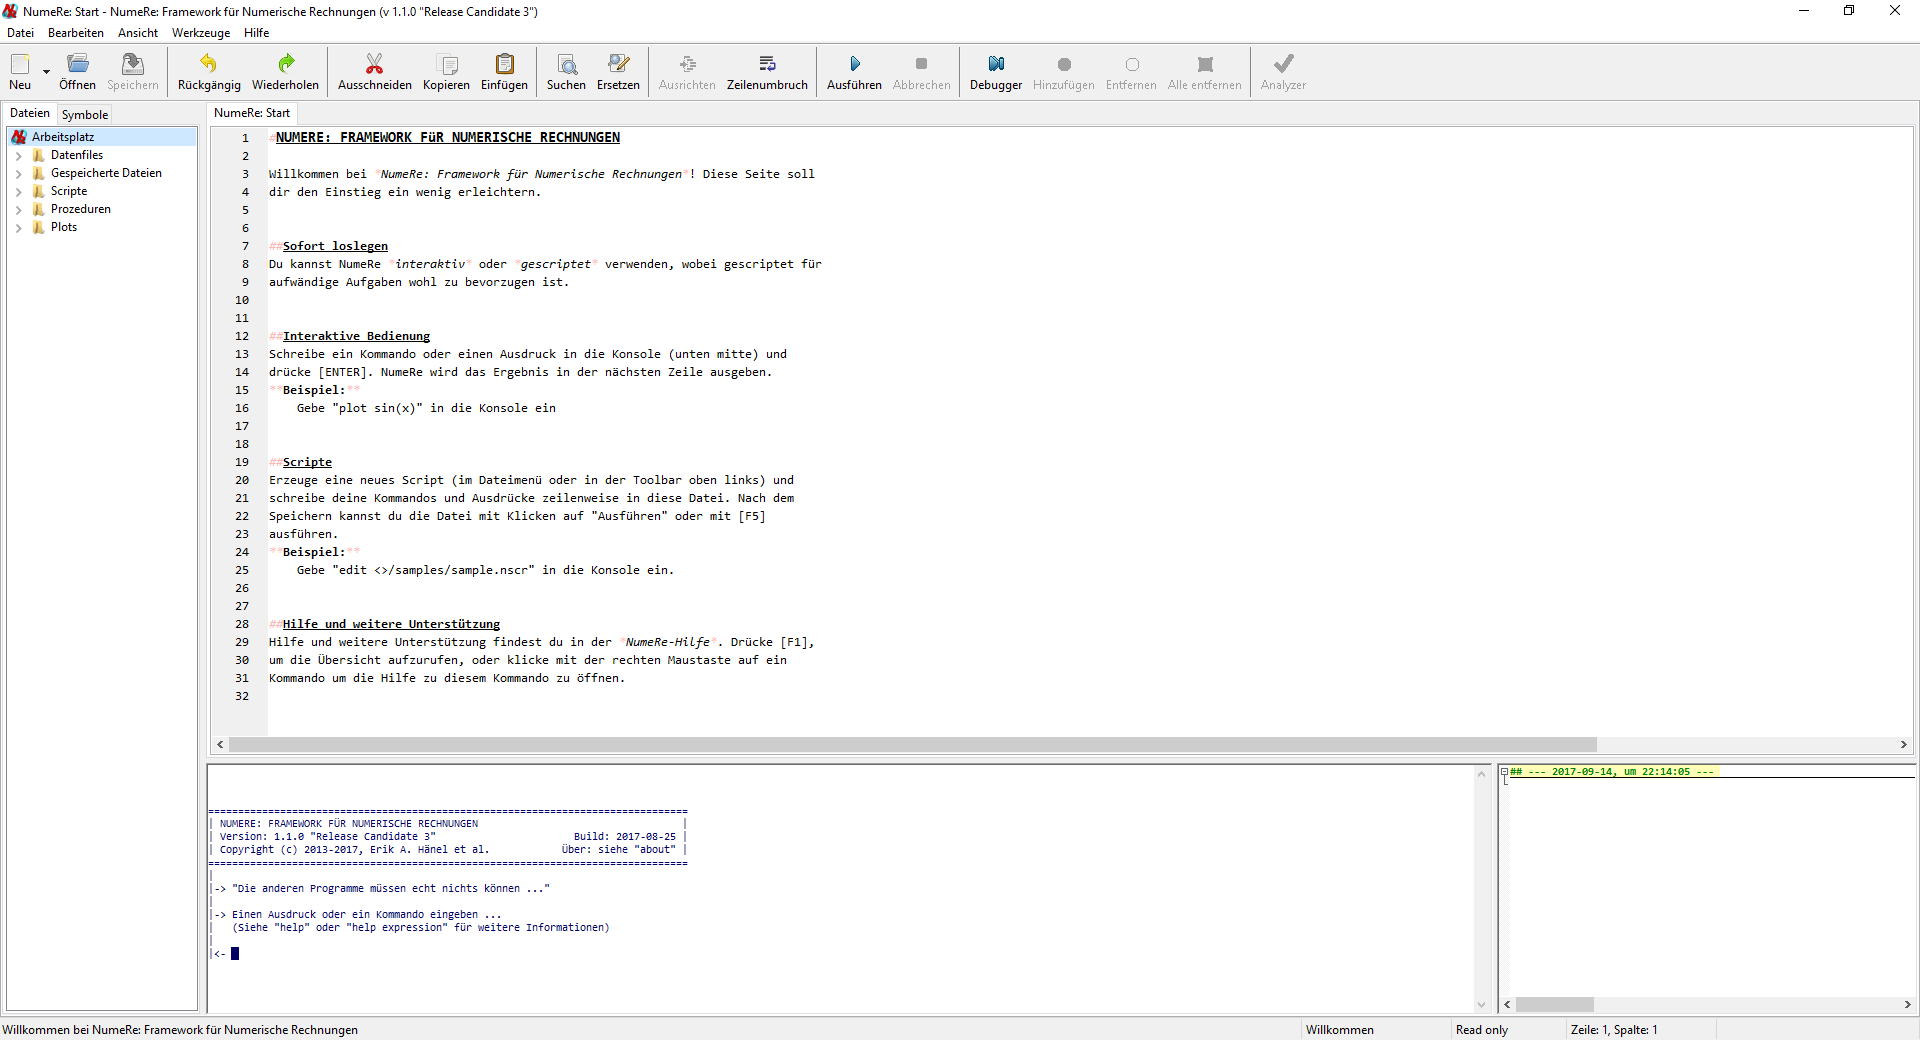
\includegraphics[width=\textwidth]{_graphics/ui.png}
					\caption{The starting view of \NR\ with the described interface elements. The starting page of \NR, which describes some basics, is also visible. \emph{Note: All screenshots shown in this document are in german language but if you've installed the english version, the interface language will be English, of course}}
					\label{fig:ui}
				\end{figure}
				The user interface of \NR\ is separated in five central elements. Most important of them is the \emph{console} (bottom center) and the \emph{editor} (top right). With the console one may interact directly with \NR\ and the editor may be used to edit text files, \NR\ scripts and \NR\ procedures. The \emph{entry history} (bottom right) is an additional element, which protocols all entries in the console, so that they may be repeated by dragging them to the console or by double clicking in them. The \emph{file tree} (left sidebar, first tab) and the \emph{symbol tree} (left sidebar, second tab) support the navigation in the files or the commands and functions, respectively. The editor itself also contains tabs, so that multiple files may be opened and edited.
				
				During the first start the \NR\ editor displays a starting page, which shall make the first task in the application more easy. Users, which are already knowing similar software (such as \textsc{Matlab}), will get familiar with these information really fast. However, we will add some first words.
				\begin{figure}[p]%
					\centering
					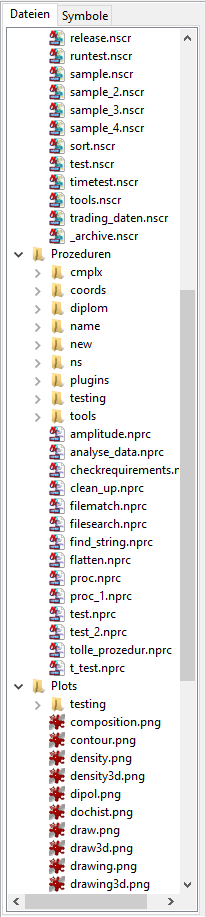
\includegraphics[width=0.2\textwidth]{_graphics/filetree.png}\hspace{5em}
					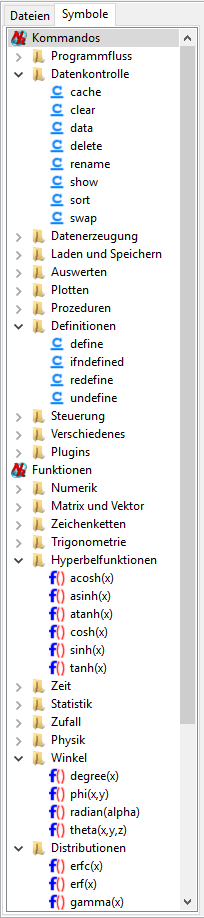
\includegraphics[width=0.2\textwidth]{_graphics/symboltree.png}
					\caption{File and symbol tree in the \NR\ interface}
					\label{fig:trees}
				\end{figure}
				First, we'll look at the interaction over the console. There's an arrow \verb+<-+ at the beginning of the line, which emphasises that an input is expected (\autoref{fig:ui}). The program's output is prefixed with an arrow, pointing in the opposite direction \verb+->+. You may \emph{only} enter something, if such an arrow (or an explicit claim) appears.
				
				\paragraph{Note}
					In a later chapter we will describe how to use loops and forks. The arrows at the beginning of the line are changing to a more special symbol. However, this is not important in this context.
				\bigskip\\
				You may enter mathematical-numerical expressions as well as commands into the \NR\ console. The syntax of the mathematical-numerical expressions is quite intuitive and will be described in the next section. The syntax of the commands has to be described more precisely.
				
				We tried to create \NR\ as intuitive as possible. This target should apply to the command syntax as well, but because \NR\ is a long-term and somehow >>grown<< application, we could not fulfill the target everywhere. However, all commands are following the same scheme:
				\begin{verbatim}
					COMMAND [EXPRESSION] [-PARAMETER[=VALUE] [OPTIONS[=VALUE]]]
				\end{verbatim}
				Syntax elements in brackets are sometimes optional or for some commands not present, respectively. Examples for the command syntax are
				\begin{lstlisting}
help
help expression
plot sin(x)
mesh sin(x)+cos(y) -set box
copy <>/samples/data* -target=<loadpath>/*
				\end{lstlisting}
				You'll recognize that (some) commands are not requiring an expression or a parameter.
				
				This command syntax is illustrated in the following sentence:
				\begin{quotation}
					\noindent\emph{>>Apply an action [on something] by using the follwing parameters.<<}
				\end{quotation}
				Applied to one of the upper examples, you can possibly say
				\begin{quotation}
					\noindent\emph{>>Open the documentation article, which has >>expression<< as topic.<<}
				\end{quotation}
				or
				\begin{quotation}
					\noindent\emph{>>Create a meshgrid plot of the function >>sin(x)+cos(y)<< by using the surrounding box.<<}
				\end{quotation}
				
				\helpidx{syntax}
				All commands are listed in the symbol tree and separated in different categories, so that the needed command may be found easily. If you dwell your mouse over a command, a tooltip will be displayed showing a short explanation. If this information is not enough, you may display the documentation article concerning the command, e.g. through\cmd{help}
				\begin{lstlisting}
help plot
				\end{lstlisting}
				All parameters and syntax information for correct execution are listed in these articles, as well as an example of the syntax.
				
				\helpidx{numere}
				If an entry is probably erroneous, \NR\ will display an corresponding message in the console. If a mathematical-numerical expression is erroneous, the position of the error---if possible---will be displayed as well. If the error results from the command syntax, \NR\ will display also a reference to the corresponding article in the \NR\ documentation.
				
				Errors in expressions or commands will abort all calculations. As a consequence all \NR\ scripts and \NR\ procedures will be aborted with an corresponding message as well.
			\section{Preferences}
				All preferences for \NR\ are set in the options dialogue, which may be found in the tools menu. Some settings may additionally be changed with the command \verb+set+. The desired setting and its new value have to follow this command:\cmd{set}
				\begin{lstlisting}
set -SETTING=VALUE
				\end{lstlisting}
				If the value of the setting shall contain whitespaces (e.g. a file path), it has to be passed surrounded with quotation marks:
				\begin{lstlisting}
set -SETTING="VALUE WITH WHITESPACES"
				\end{lstlisting}
				The command \verb+list+ may display a list of all preferences:\cmd{list}
				\begin{lstlisting}
list -settings
				\end{lstlisting}
				All default preferences of \NR\ are in principle set reasonable.
				
				Changed settings are saved at application termination and available again after a restart.
			\section{Simple Calculations}
				As a framework for numerical calculations, \NR\ may of course calculate numerically. The equations, which shall be evaluated, may be entered similar to a pocket calculator. Spaces between operators and values don't play any role, but there are \emph{no spaces} allowed between function names and their argument parentheses. Lower- and uppercase letters are of course different and the multiplication dot \verb+*+ mustn't be omitted:
				\begin{lstlisting}
5*cos(_2pi)
				\end{lstlisting}
				multiplies $\cos2\pi$ with 5 and returns the result in the next line. The value \verb+_2pi+ is a built-in constant for $2\pi$ and \verb+cos()+ is of course the cosine function.

				The built-in constants and functions may be found in the symbol tree. They may be found as well by entering 
				\begin{lstlisting}
list -const
list -func
				\end{lstlisting}
				into the console. \verb+list -func+ may also be restricted further.
				
				\helpidx{list}
				\NR\ cannot only handle numbers but also variables. The variables \verb+x+, \verb+y+, \verb+z+, \verb+t+ and \verb+ans+ are already predefined. However, you may define more variables for the current session. This is done either automatically (if \NR\ stumbles upon an unknown variable) or through and explicit assignment:
				\begin{lstlisting}
neue_variable = 5
				\end{lstlisting}
				(\emph{This variable's name is german for staying consistent with the screenshots.}) This line declares the new variable \verb+neue_variable+ and assigns the value 5 to it. The upper equation may now be written as follows:
				\begin{lstlisting}
neue_variable*cos(_2pi)
				\end{lstlisting}
				
				\NR\ may as well evaluate multiple expressions simultaneous. The expressions have to be separated by a comma \verb+,+. In the whole (multiple) expression line, \NR\ will evaluate the values from left to right. The line
				\begin{lstlisting}
neue_variable = 5, neue_variable*cos(_2pi), neue_variable = 1
				\end{lstlisting}
				assigns 5 to \verb+neue_variable+, calculates $5\cos2\pi$ and finally assigns 1 to \verb+neue_variable+ (\autoref{fig:first_calc_1}). This way of writing a calculation may be speed up the evaluation inside of loops significantly.
				
				\helpidx{expression}
				\begin{figure}[htb]%
					\centering
					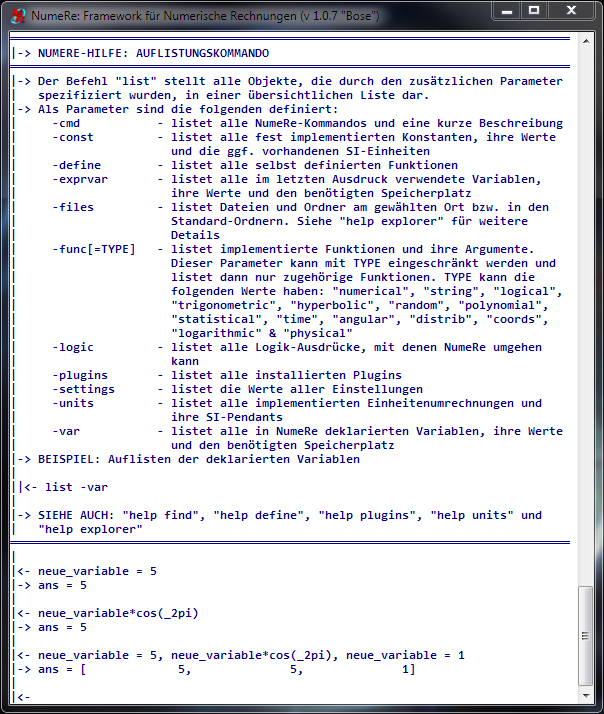
\includegraphics[width=\textwidth]{_graphics/first_calc_1.png}
					\caption{\NR\ after the evalution of the last calculation. You may notice that the input is as well stored in the entry history}
					\label{fig:first_calc_1}
				\end{figure}
			\section{Important Commands}
				You will interact with \NR\ mainly with commands. The most important commands are\cmd{help\\find\\list\\quit}
					\begin{lstlisting}
help
help TOPIC
find TERMS
list -OBJECT
					\end{lstlisting}
					These commands call the integrated documentation (\verb+help+ or \verb+help TOPIC+ for the desired topic, respectively), the keyword search (\verb+find TERMS+) and list objects (\verb+list -OBJECT+).
					
					All commands have an entry in the \NR\ documentation. This article may be read by entering \verb+help COMMAND+ into the console or by using the corresponding item in the context menu and contains all necessary information about the command and---if applicable---references to further important articles. In the case that an information may not be found direclty in the \NR\ documentation, you may use the keyword search (\verb+find+), which will also return the corresponding articles in the \NR\ documentation.
					\paragraph{Note}
						By using a semicolon >>\verb+;+<< you may also enter multiple commands and expressions, which shall be evaluated successively, in a single line:
						\begin{lstlisting}
COMMAND1; COMMAND2; EXPRESSION1; COMMAND3; EXPRESSION2; ...
						\end{lstlisting}
		\chapter{Loading and Using Data}
			One of the main tasks in scientific work is data analysis. Therefore it is necessary to use applications, which may load and process the corresponding large amout of data in a reasonable time frame. \NR\ transforms all read data into a table and may calculate statistics, histograms and more elaborate evaluations.
			\section{File Types}
				In addition to simple text files in ANSI format (using the file extensions *.txt and *-dat) \NR\ can load the following file formats:
				\begin{itemize}
					\item \textbf{CassyLab file (*.labx).} This file type is only used by CassyLab and contains a complete CassyLab experiment. However, \NR\ will only extract the data table.
					\item \textbf{CSV file (*.csv).} Comma-Separated-Values files are a nearly-standard for data exchange. However, there is no real >>CSV standard<< defined, so that though tested it is possible that \NR\ cannot read single CSV files correctly. (Please notify the programmer if you face such a problem and forward him the file.)
					\item \textbf{JCAMP-DX file (*.dx, *.jdx and *.jcm).} JCAMP-DX files (meaning \emph{Joint Committee on Atomic and Molecular Physical data -- Data eXchange}) are a standard for file exchanges of spectroscopy data. \NR\ will only extract the data table out of these files.
					\item \textbf{OpenDocument spreadsheet (*.ods).} These are data tables, which are created for example by OpenOffice Calc. \NR\ can only extract the real numerical and string values but not the equations. Please note also that files opened with OpenOffice Calc are locked: these spreadsheets are not readable by \NR.
					\item \textbf{Excel workbooks (*.xls and *.xlsx).} These are data tables, whcich are created by Excel. \NR\ will only extract the numerical and string values, not the equations. The legacy Excel format also doesn't provide the values calculated by the equations in the data tables, so that these are not available in this case. Please note also that files opened with Excel are locked: these workbooks are not readable by \NR.
					\item \textbf{IGOR Binary Waves (*.ibw).} IGOR Binary Waves contain the data of a (1, 2 or 3 dimensional) IGOR wave.
					\item \textbf{NumeRe data file (*.ndat).} NumeRe data files are a data format by \NR, which is used for fast saving and loading of data sets.
				\end{itemize}
				
				\helpidx{load}
				However, \NR\ may not write all of these formats. The following output formats are available:
				\begin{itemize}
					\item \textbf{Text file (*.dat or *.txt).} \NR\ creates a text file in ANSI encoding, which is following the formatting standards in the next section. Most of the other applications should be able to read these files
					\item \textbf{NumeRe  data file (*.ndat).} This file format can only be read by \NR. However, this file format is documented online and may implemented in other programs.
					\item \textbf{CSV file (*.csv).} \NR\ creates a CSV file, where commas \verb+,+ are used as column and dots verb+.+ are used as decimal separators. (Some table calculations, especially those, which are using the comma as decimal separator, probably cannot read these files: if you replace the commas with semicolons \verb+;+ and the dots with commas, this problem should be fixed. The programmer does not understand this behavior.)
					\item \textbf{Excel Workbook (*.xls).} \NR\ may write the data in the legacy Excel-(97-2003)-Format (*.xls) for further processing in Excel and similar applications.
					\item \textbf{\TeX\ file (*.tex).} \NR\ writes a table using the \TeX\ standard. The comments in this file contain the preconditions for including the table in a \TeX\ document (\emph{booktabs} and \emph{longtable} Packages).
				\end{itemize}
				
				\helpidx{save}
			\section{Formatting of Text Files}
				Although \NR\ uses the dot \verb+.+ in the console as decimal separator, it is not necessary for files. \NR\ may even read files, which are using the comma and the dot mixed. All commas are transformed to dots internally.
				
				However, text files have to be formatted as a table. It is not relevant, if the columns of this file are separated using whitespaces, tabulators or a mixture of both.
				
				If you have text inside of the data table, it will be ignored. If you want to provide a column header, you have to put these headers in the last line before the actual data. Whitespaces in a single column header have to be replaced with underscores \verb+_+. If you want to provide some comments in this file, prefix that with a \verb+#+ at the beginning of the line (Column headers are found even it they are prefixed with a \verb+#+). You may also use a separating line between the column headers and the data table made out of \verb+=+.
				\begin{verbatim}
					# COMMENT
					# COMMENT
					# HEAD_1  HEAD_2  HEAD_3 [...]
					# =======================[...]
					   0,225      12       0 [...]
					   0,245    12.5      .5 [...]
				\end{verbatim}
				
				\helpidx{data}
			\section{Loading and Using of Files}
				You may load the file in the previously defined formats, if you drag and drop them on the console, use the corresponding item in the context menu of the file tree and through\cmd{load}
				\begin{lstlisting}
load FILEPATH/FILE.EXT
				\end{lstlisting}
				File paths and file names containing whitespaces have to be surrounded with quotation marks. The exemplary \verb+FILEPATH+ may be omitted, if the file is located in the default directory \verb+<loadpath>+ (which is---as default---the folder >>data<< in the \NR\ root directory). If the file extension \verb+.EXT+ is omitted, \NR\ will interpret that as an text file with the foile extension *.dat. There is further information on this topic in the \NR\ documentation at \verb+help load+.
				
				There are some example files in the subdirectory >>samples<< in a default \NR\ installation. You may load them for example through
				\begin{lstlisting}
load <>/samples/data
				\end{lstlisting}
				The symbol \verb+<>+ is a path placeholder, which points to the \NR\ root directory. This line loads the file >>data.dat<< to \NR's memory. The data is now available as a table in the data object \verb+data()+ and may be used (It is a coincidence that the file and the data object carry the same name. The data of loaded files is always stored to \verb+data()+).
				
				You may display the data table with the command \verb+show+:\cmd{show}
				\begin{lstlisting}
show data()
				\end{lstlisting}
				This will display the table in a separate window.
				
				You may access the data in \verb+data()+ using the so-called \emph{interval syntax} \verb+a:b+ (for values ranging from \verb+a+ to \verb+b+). This is used to define the column and row ranges, from where the data should be taken. You pass these indices inside of the argument parentheses of \verb+data()+:\cmd{data()}
				\begin{lstlisting}
data(3,1)
data(:,1)
data(4:55,4)
data(3,3:)
				\end{lstlisting}
				In these examples a single element is selected (\verb+data(3,1)+ for third row and first column), a whole column (\verb+data(:,1)+ for all rows in the first column), a subselection of a column (\verb+data(4:55,4)+ for fourth to 55th row and fourth column) or a subsection of a row (\verb+data(3,3:)+ for third row and third to last column).
				
				You only may extract values using columns or rows inside of calculations, i.e. the interval syntax may only be used for rows or columns. It is not possible to perform calculations using subtables, however, you may use the matrix operations out of a later chapter to achieve this behaviour. However, you may use different elements of \verb+data()+ in a single expression:
				\begin{lstlisting}
(cos(data(:,1)) + sin(data(:,2))) * sqrt(data(1,3:))
				\end{lstlisting}
				This expression will return as many elements as the longest interval nominates. There are also functions, which can handle an arbitrary number of elements and calculate a single result:
				\begin{lstlisting}
avg(), cmp(), cnt(), max(), med(), min(), norm(), num(), prd(), std(), sum(), to_char()
				\end{lstlisting}
				These functions calculate statistics of the elements (average, median, standard deviation, minimal and maximal value), summarize or multiply their arguments, search for elements, count elements or transform the values to ASCII character codes (the usage of strings is explained in the part >>Advanced Usage<< and is not relevant at this point).
				
				\paragraph{Note}
					Users, who are already familiar with Matlab or Octave, will know the difference between \verb+OPERATOR+ and \verb+.OPERATOR+. This doesn't exist in \NR, because \NR\ was completely designed as a table calculation. Elements from different columns or lines will always be processed element by element and not following a matrix or vector algebra (a matrix-matrix or a matrix-vector multiplication is provided by the framework in the context of the \verb+matop+ command using the \verb+**+ operator).\bigskip\\
				Some commands, like \verb+fit+, \verb+fft+ and \verb+plot+ (and similar) can handle whole subtables. In the context of this commands you may use the interval syntax in both, columns and rows.
				
				The table in \verb+data()+ is a so-called \emph{read-only} data set. This means that the data in this table may not be overwritten or modified in other means. In a later chapter we will explain the caches as tables, which may be manipulated.
				
				\helpidx{data}
			\section{Data Analysis}
				The data analysis is probably the main reason, why someone should search for a fast and simple numerics application. \NR\ provides many predefined functions for analysis, which may be used fast and mostly uncomplicated. The needs for the most common statistics should be fulfilled satisfyingly.
				
				You may either calculate the statistics all at once with the command \verb+stats+\cmd{stats}
				\begin{lstlisting}
stats data(i1:i2,j1:j2)
				\end{lstlisting}
				or single with the statistical functions, which where mentioned in the previous section:
				\begin{lstlisting}
std(data(i1:i2,j1))
avg(data(i1:i2,j1))
[...]
				\end{lstlisting}
				The command \verb+stats+ returns nearly all reasonable statistical value of the table, which is for example the average, the standard deviation and the standard error, RMS, skewness, excess and the student factor (for a two-fold 95 \%\ confidence interval). Most of them can also be calculated through single functions.
				
				\helpidx{stats}
				A very common way of analyzing a data set is generating a histogram. Histograms are a way to visualize the frequency of a measured quantity. This may either be the period of a oscillation, or the life time of elementary particles or another quantity.
				\begin{figure}[htb]%
					\centering
					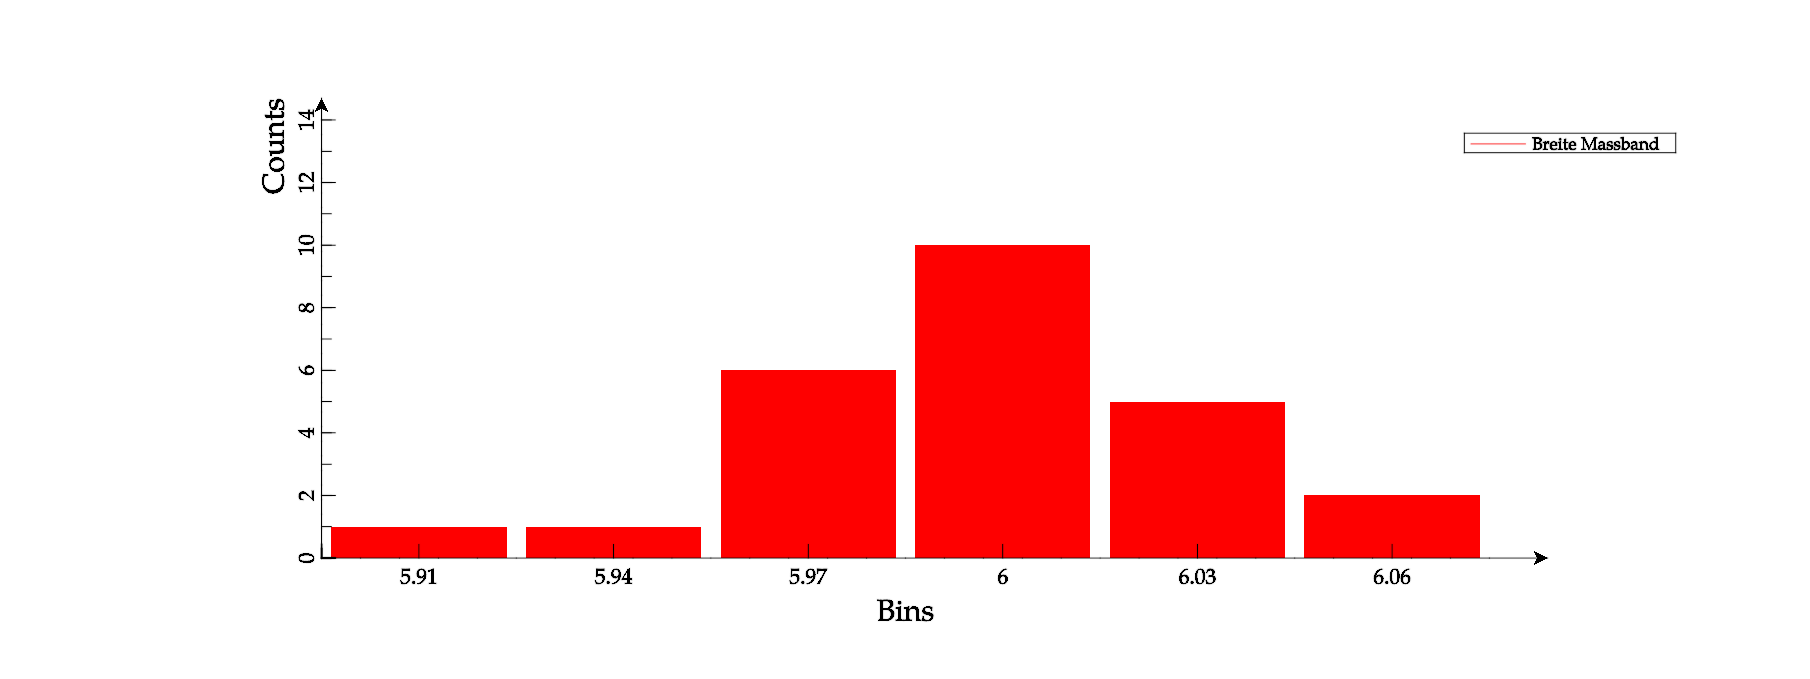
\includegraphics[width=\textwidth]{_graphics/histogramm.png}
					\caption{Histogram of a data set, which was created using \texttt{hist}}
					\label{fig:histogramm}
				\end{figure}
				
				Histograms of the loaded data are created using \cmd{hist}
				\begin{lstlisting}
hist data(i1:i2,j1:j2)
				\end{lstlisting}
				The command \verb+hist+ supports a large number of parameters, which may modify the created histogram even further, though the results without any parameters are already good (\autoref{fig:histogramm}). The number of used bins is determined by the \emph{Rule of Sturges}, but may also be set directly or based upon the \emph{Rule of Scott} or the \emph{Rule of Freedman and Diaconis}.
				
				A histogram is calculated for each column of the data set and the results are presented in a common graph. Columns, which don't contain any reasonale data, have to be excluded using the interval syntax.
				
				\NR\ may also calculate histograms out of a two-dimensional data set. You either have to pass the option \verb+grid+ for a single histogram or the command \cmd{hist2d}\verb+hist2d+ for histograms in two spatial directions. Futher details are listed in the corresponding documentation article.
				
				\helpidx{hist}
				One additional, very common way of analyzing data next to histograms and statistics is to fit a function (sometimes called \emph{model} or \emph{regression curve}) to the measured (and already somehow processed) data.
				
				To fit a function \verb+FUNCTION()+ to data in \verb+data()+, you can use the command \verb+fit+:\cmd{fit}
				\begin{lstlisting}
fit data(:,j1:j2) -with=FUNCTION(x,PARAMS) params=[PARAMS=INITIALW.]
fit data(:,1:2) -with=A*sin(B*x+C) params=[A=1,B=1,C=0]
				\end{lstlisting}
				\NR\ will now try to alter the parameters \verb+PARAMS+ in a way that the \verb+FUNCTION()+ matches the data points best. The fitted values are stored in the parameters so that you can continue your calculations with these values directly. (In newer \NR\ versions it os not necessary to provide the parameters through \verb+params+. \NR\ will detect them on its own.)
				
				If \NR\ reaches an optimal set of parameters, it will cancel the algorithm and return an overview of the parameters, which is presented as an example in the following:
				\begin{verbatim}
					Function: 0.646875*sin(3.00223*x+0.00837336)
					Data points:                            101 without weighting factors
					Degrees of freedom:                     98
					Parameters for the algorithm:           TOL=0.0001, MAXITER=500
					Iterations:                             7
					Weighted sum of the residuals (chi^2):  2.33825
					Variance of the residuals (red. chi^2): 0.0238597
					Standard deviation of the residuals:    0.1544658

					Parameter  Initial value        Fitted        Asymptotic standard error
					-----------------------------------------------------------------------
					A                      1     0.6468754    ± 0.02188576         (3.383%)
					B                      3      3.002228   ± 0.005649476        (0.1882%)
					C                      0   0.008373364    ± 0.06579646         (785.8%)
					----------------------------------------------------------------------

					Correlation matrix of the fitted parameters:

					/          1     0.0159    -0.0164 \
					|     0.0159          1     -0.862 |
					\    -0.0164     -0.862          1 /

					Fitting result analysis:
					The fitted function could describe the trend of the data points, but 
					there is some room for optimisation.
				\end{verbatim}
				This overview contains the important quantity $\chi^2$, which contains the sum of the quadratic deviations of the data points to the fitted function. In addition, you'll find the result values of the parameters and the calculated error values, which may inserted in the concluding error progression. The correlation matrix of the parameters contains an information, how the parameters are connected to each other and the fitting result analysis is a summary of what can be learned from the value of $\chi^2$. This overview will also be stored in the fit log file at \verb+<savepath>/numerefit.log+.
				\begin{figure}[htb]%
					\centering
					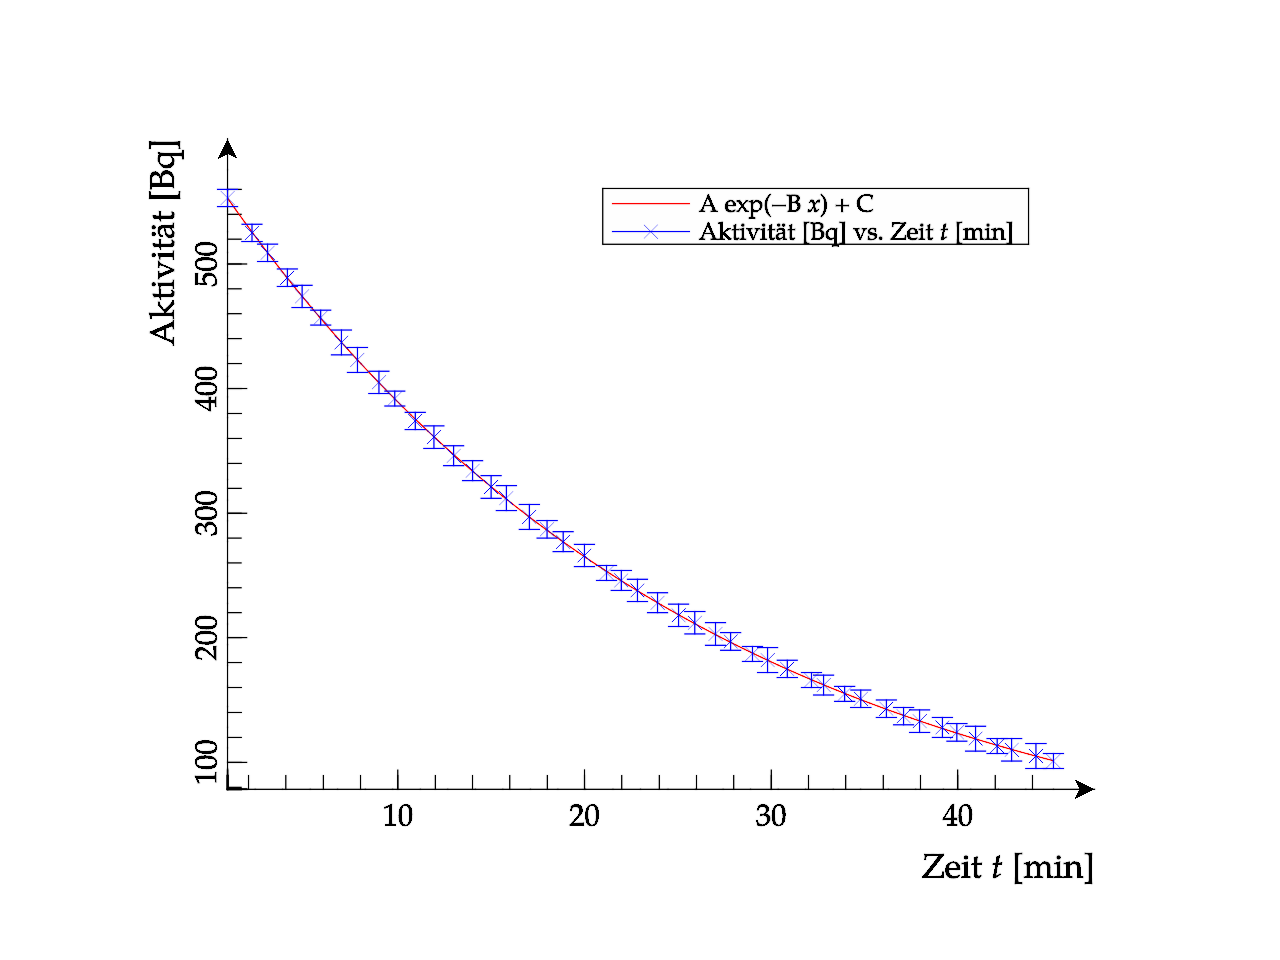
\includegraphics[width=\textwidth]{_graphics/plot.png}
					\caption{Fitting a model for an exponential decay with \texttt{fitw}}
					\label{fig:fit}
				\end{figure}
				
				\paragraph{Note}
					If the quantity $\chi^2$ is an indicator on the quality of the fit, can be discussed. In common, one assumes that a fit with the smallest possible $\chi^2$ value has the best possible parameter set. More precise: it's the so-called reduced $\chi^2$ value, which is the important quantity: if it is noticeable smaller than 1, the resulting parameter set seems to fit the data points quite well. If you perform a fit, which will consider the error estimations (see below), this value should be in the range of 1. \NR\ will consider all these conditions and return a corresponding fitting result analysis. But note that the analysis may only support and not fully replace the optical comparation of fitted function and data points.\bigskip\\
				After the fitting procedure, the fitted function may be displayed graphically using the command \verb+plot+ (see next chapter) (\autoref{fig:fit}). This is a good possibility to check the results of the fitting procedure (and should always be performed).
				
				If you can estimate the measurment errors, \NR\ may consider these values. Just use\cmd{fitw}
				\begin{lstlisting}
fitw data(:,1:2:3) -with=A*sin(B*x+C) params=[A=1,B=1,C=0]
				\end{lstlisting}
				\verb+fitw+ (for \emph{weighted fit}) uses the error estimations in the third column to calculate the weighting factors for the data points: data points with higher errors are considered less important than those with small errors.
				
				If a fitting procedure does not converge, it may help varying the initial values of the parameters (which shall be passed everytime). It also may help to restrict the fitting interval. This may be done either through restricting the rows in \verb+data()+ or through passing the option \verb+x=a:b+:
				\begin{lstlisting}
fit data(:,1:2) -with=A*sin(B*x+C) params=[A=1,B=1,C=0] x=0:4
				\end{lstlisting}
				In addition the maximal number of iterations, the precision and further restrictions of the parameters can be set. The last option may have a large influence on the stability of the algorithm.
				
				\helpidx{fit}
				All mentioned commands are acting along the columns. If the data is organized in rows, one has to perform the following line\cmd{copy}
				\begin{lstlisting}
copy data(:,:) -target=cache(:,:) transpose
				\end{lstlisting}
				and replace \verb+data+ with \verb+cache+ in all previous examples.
		\chapter{Creating Graphs}
			A very important functionality of \NR\ is the creation of function and data graphs. You may visualize the behaviour of functions and data and analyze them more easy. \NR\ can store all created graphs in image files, if you specify that in the options list of the graph.
			\section{Types of Graphs}
				\NR\ knows a large number of different plot types, which may be modified further by passing further options to the options list. The following list shall only mention the most important plot types. You can get the full list by entering the command \verb+list -cmd+:
				\begin{lstlisting}
plot
plot3d
mesh
dens
vect
vect3d
...
				\end{lstlisting}
				\begin{itemize}
					\item \verb+plot+: this creates a standard graph, which displays $y$ against $x$. This command is being used, if you want to visualize $\sin x$ or $x^2$.
					\item \verb+plot3d+: this command creates a graph on the basis of a 3-dimensional trajectory. A trajectory is calculated from three functions sharing the variable $t$ and visualized three-dimensionally.
					\item \verb+mesh+: a function $z = f(x,y)$ may be displayed with this command. A meshgrid is calculated and displayed three-dimensionally.
					\item \verb+dens+: this command visualizes the function $z = f(x,y)$ in contrast to \verb+mesh+ only through colour values projected to the $x$-$y$ plane.
					\item \verb+vect+: this plotting style calculates a vector plot of a 2D vector field: $\vec A(x,y) = A_x(x,y)\,\hat e_x + A_y(x,y)\,\hat e_y$.
					\item \verb+vect3d+: this calculates a vector plot similar to \verb+vect+, but it uses a three-dimensional vector field as data basis: $\vec A(x,y,z) = A_x(x,y,z)\,\hat e_x + A_y(x,y,z)\,\hat e_y + A_z(x,y,z)\,\hat e_z$.
				\end{itemize}
			\section{Output}
				The default output channel for plots is the \NR\ GraphViewer, in which the plots may be modified further. Additionally, the plots may be stored into an image file in the PNG format in the directory \verb+<plotpath>+ (This is per default the subdirectory >>plots<< in the \NR\ root). You may change the image file format to othe formats. This may be done with the plotoptions \verb+opng+, \verb+oeps+, \verb+ogif+, \verb+osvg+ and \verb+otex+.
				
				To create a simple plot in for example >>graph\_of\_the\_measurement.png<<, you've to pass the option
				\begin{lstlisting}
opng=graph_of_the_measurement
				\end{lstlisting}
				If the file name of the target file shall contain whitespaces, you've to pass it in enclosing quotation marks.
				
				\helpidx{plotoptions}
			\section{Usage}
				The syntax of all plotting commands is following this scheme:
				\begin{lstlisting}
COMMAND FUNCTIONS/DATA -set OPTIONS
				\end{lstlisting}
				where \verb+OPTIONS+ are optional and may be omitted.

				Default variables are $x, y, z$ and $t$. Depending on the actual plotting command, one, two, three or all four of these variables are used as plotting variables and the others are parameters. \verb+plot+ uses only $x$, \verb+plot3d+ only $t$, \verb+mesh+, \verb+dens+ and \verb+vect+ $x$ and $y$ and \verb+vect3d+ uses $x, y$ and $z$. All other variables are parameters.
				
				A simple plot of a sine is created with\cmd{plot}
				\begin{lstlisting}
plot sin(x)
				\end{lstlisting}
				This calculates a sine function from $-10$ to $10$ automatically, where the $y$ axis was chosen fitting but a small amount larger than the minimal and maximal value of the function. The axis labels and the legend are also determined automatically (\autoref{fig:sinusplots}a)
				\begin{figure}[p]%
					\centering
					\subfloat[without options]{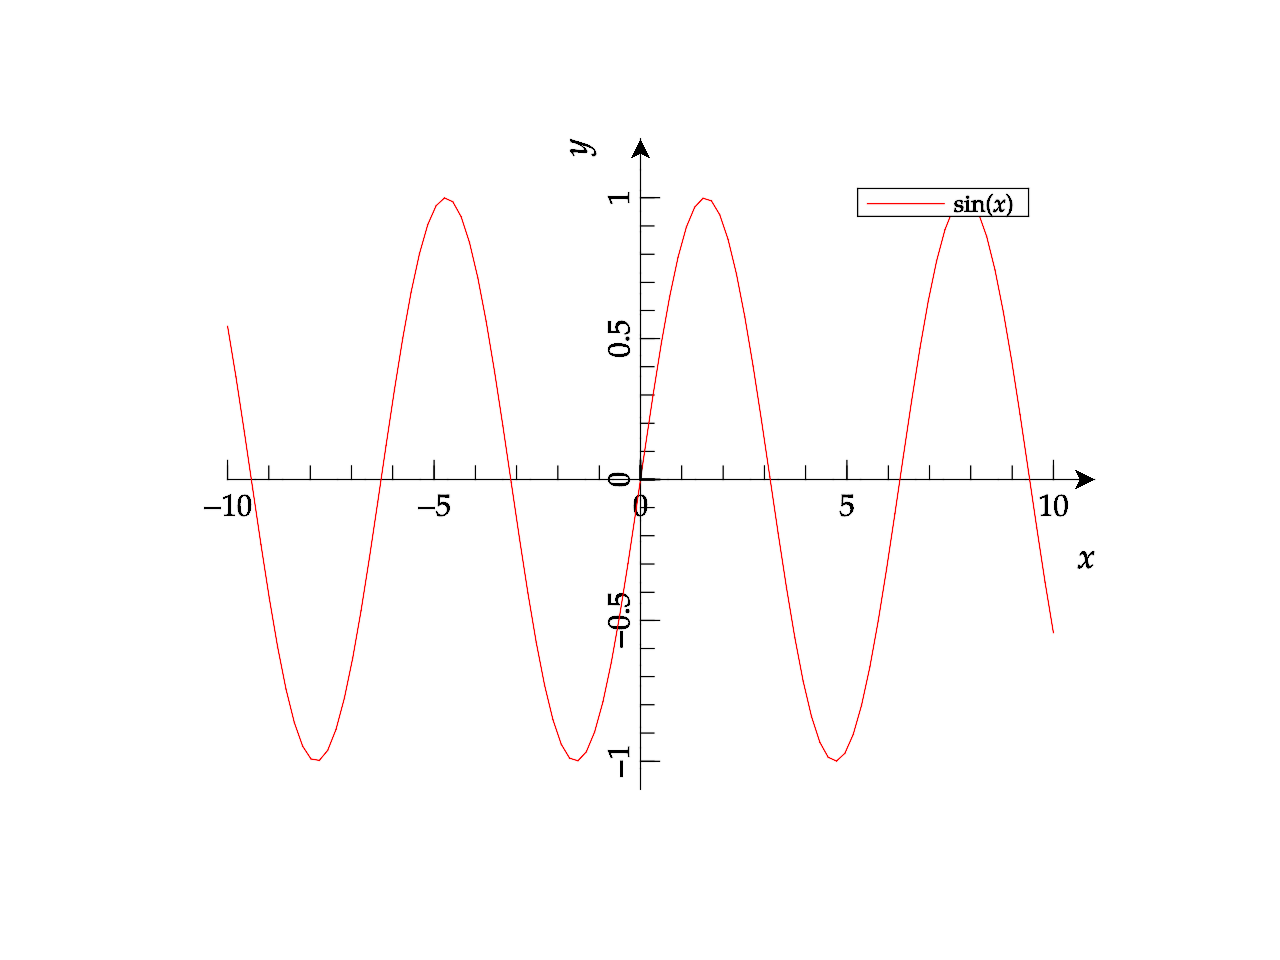
\includegraphics[width=0.45\textwidth]{_graphics/plot_0.png}}
					\subfloat[with \texttt{box} and \texttt{grid}]{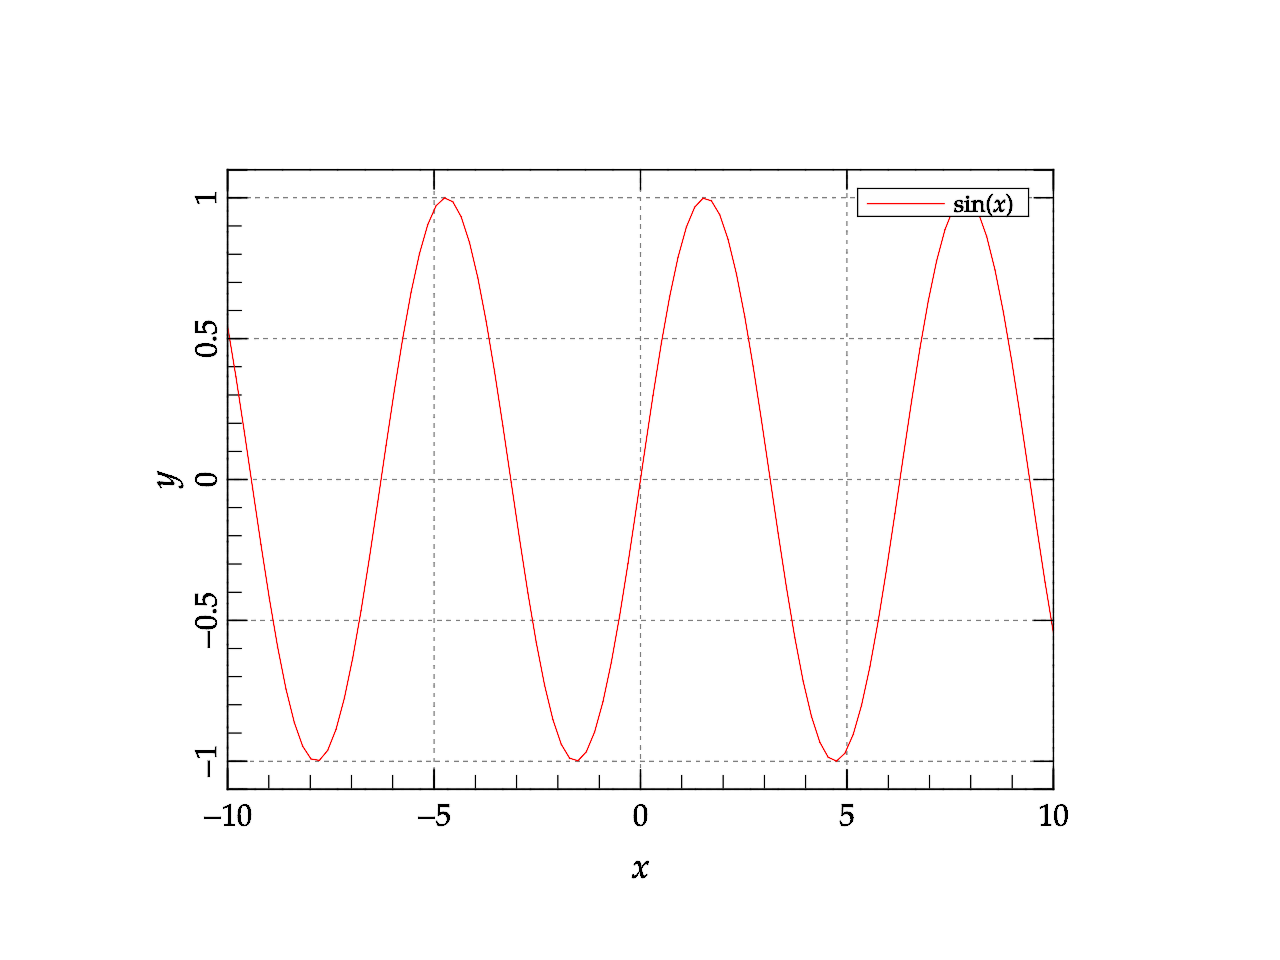
\includegraphics[width=0.45\textwidth]{_graphics/plot_1.png}}\\
					\subfloat[with custom legend]{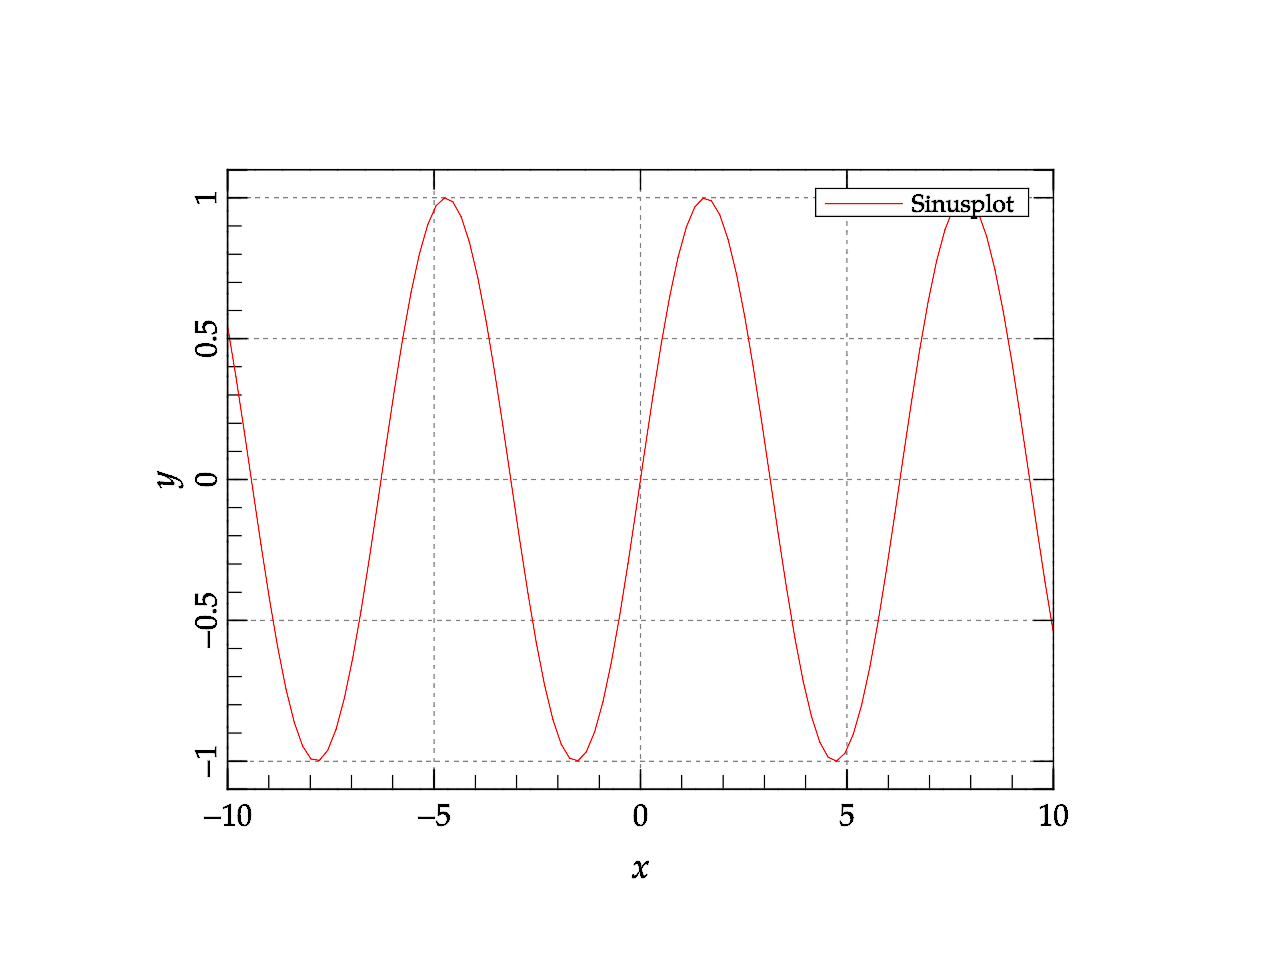
\includegraphics[width=0.45\textwidth]{_graphics/plot_2.png}}
					\subfloat[with data set]{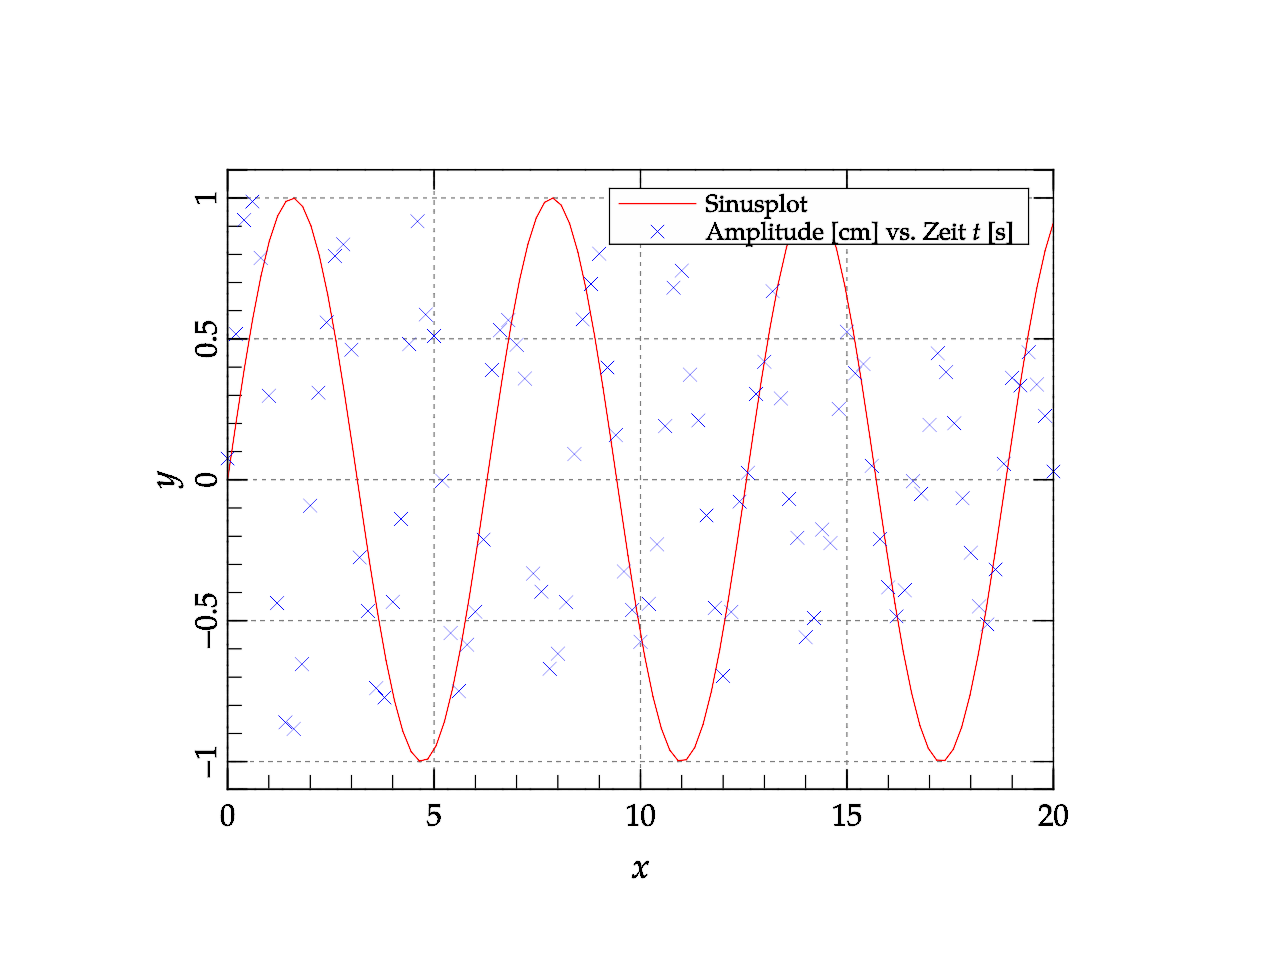
\includegraphics[width=0.45\textwidth]{_graphics/plot_3.png}}\\
					\subfloat[with custom interval]{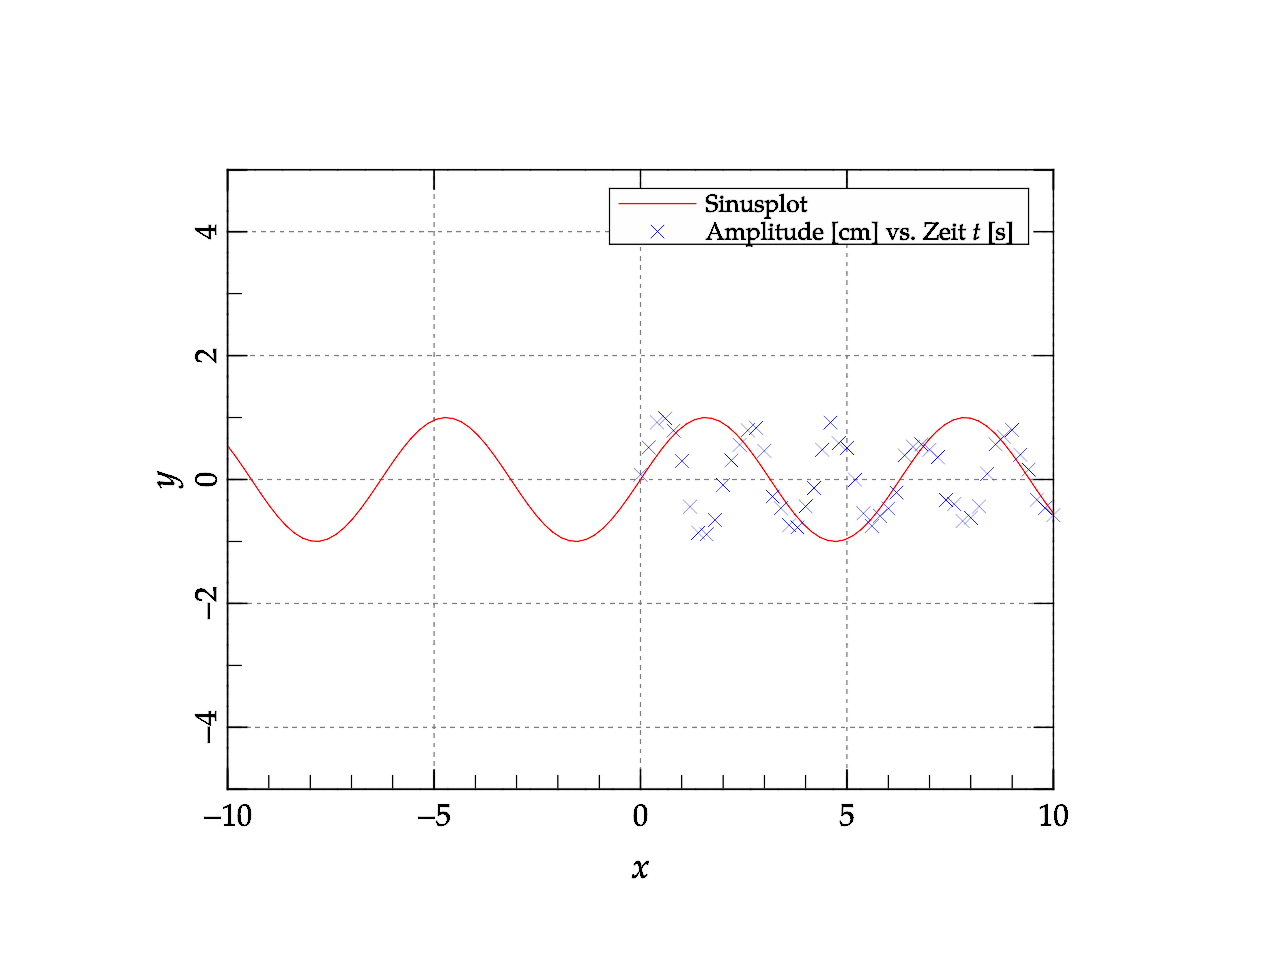
\includegraphics[width=0.45\textwidth]{_graphics/plot_4.png}}
					\subfloat[with errorbars]{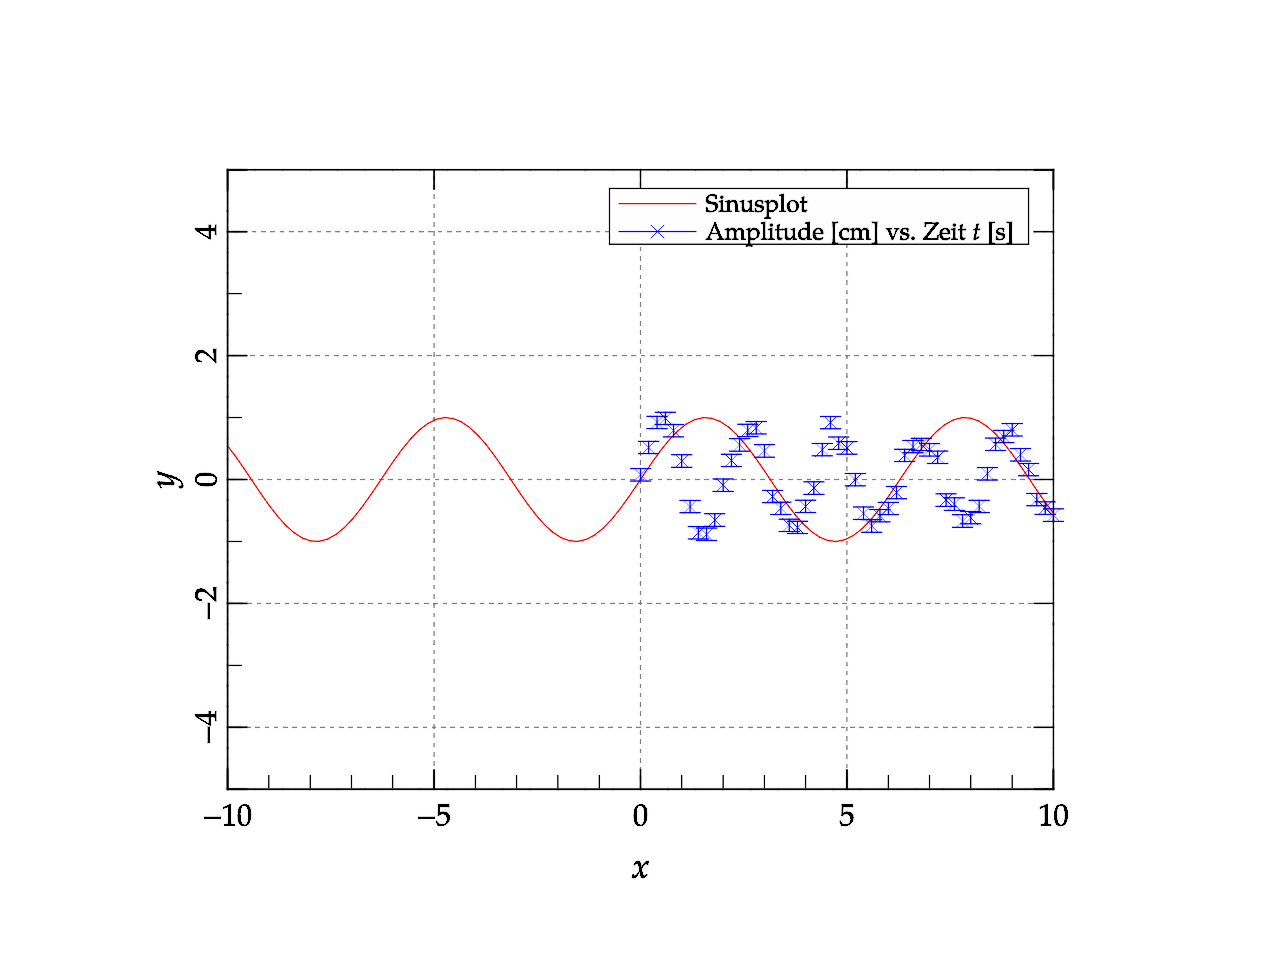
\includegraphics[width=0.45\textwidth]{_graphics/plot_5.png}}
					\caption{The resulting graphs using the shown options}
					\label{fig:sinusplots}
				\end{figure}
				
				\helpidx{plot}
				You are getting a surrounding box and a coordinate grid with 
				\begin{lstlisting}
plot sin(x) -set box grid
				\end{lstlisting}
				This and all further plots will also get a grid and a box (\autoref{fig:sinusplots}b and c).
				
				If you want to have >>Sine function<< instead of >>$\sin(x)$<< as legend, you'll have to enter the following:
				\begin{lstlisting}
plot sin(x) "Sine function" -set box grid
				\end{lstlisting}
				(\autoref{fig:sinusplots}c; An empty legend is achieved by passing an empty string \verb+""+)
				
				\NR\ may also display data points graphically. To achieve this, one has to pass the data set in \verb+data()+ analogous to a function. If you leave the argument's parentheses empty, this will be replaced automatically with \verb+data(:,:)+. You may also specify the desired columns by yourself, e.g. \verb+data(:,1:4)+. \NR\ will use either the columns 1 and 4 or the columns 1 to 4, if the corresponding plotting style needs more than two columns. You may specify up to six columns in an arbitrary order: \verb+data(:,4:2:6:1:3:8)+.
				
				In combination with the previous example, one may visualize the columns 1 and 2 together with the sine function through
				\begin{lstlisting}
plot sin(x) "Sine function", data() -set box grid
				\end{lstlisting}
				(\autoref{fig:sinusplots}d). Even for \verb+data()+ one may pass a customn legend. Otherwise \NR\ will create a combination of the columns titles. Additional it's noticable that adding the data set has scaled the $x$ axis corresponding to the data set. Also noticeable is that \NR\ displays the data points as single points and doesn't connect them with a (non-physical) line.
				
				The plotting intervals may be overwritten for a plot, if they are passed explicitly:
				\begin{lstlisting}
plot sin(x) "Sine function", data() -set box grid [-10:10,-5:5]
				\end{lstlisting}
				This creates a graph with the $x$ interval $[-10;10]$ and the $y$ interval $[-5;5]$ (\autoref{fig:sinusplots}e). This option will \emph{not} be used for successive plots.
				
				Measurements of data points are often combined with measurement errors. If these are known, \NR\ may display them correspondingly. If only the $y$ values have errors, \NR\ needs three columns ($x,y,\Delta y$), if both directions have errors, \NR\ will need four ($x,y,\Delta x, \Delta y$). The needed plotting option is \verb+errorbars+ or \verb+yerrorbars+, if only $y$ errors are available.
				
				If wie assume that the data points in the upper example have errors in $y$ direction, we may enter:
				\begin{lstlisting}
plot sin(x) "Sine function", data() -set box grid [-10:10,-5:5] yerrorbars
				\end{lstlisting}
				Errorbars in $y$ direction are appearing, although the number of columns was not changed! \NR\ interprets the empty argument's parenthesis now automatically in another way and uses the first three columns (\autoref{fig:sinusplots}f).
				
				\helpidx{plotoptions}
				\cmd{mesh}In another case a two-dimensional function shall be visualized using a meshgrid plot: the function is the cardinal sine of $\varrho$ ($\text{sinc}\,\varrho$):
				\begin{lstlisting}
mesh sinc(norm(x,y))
				\end{lstlisting}
				\begin{figure}[p]%
					\centering
					\subfloat[only \texttt{mesh}]{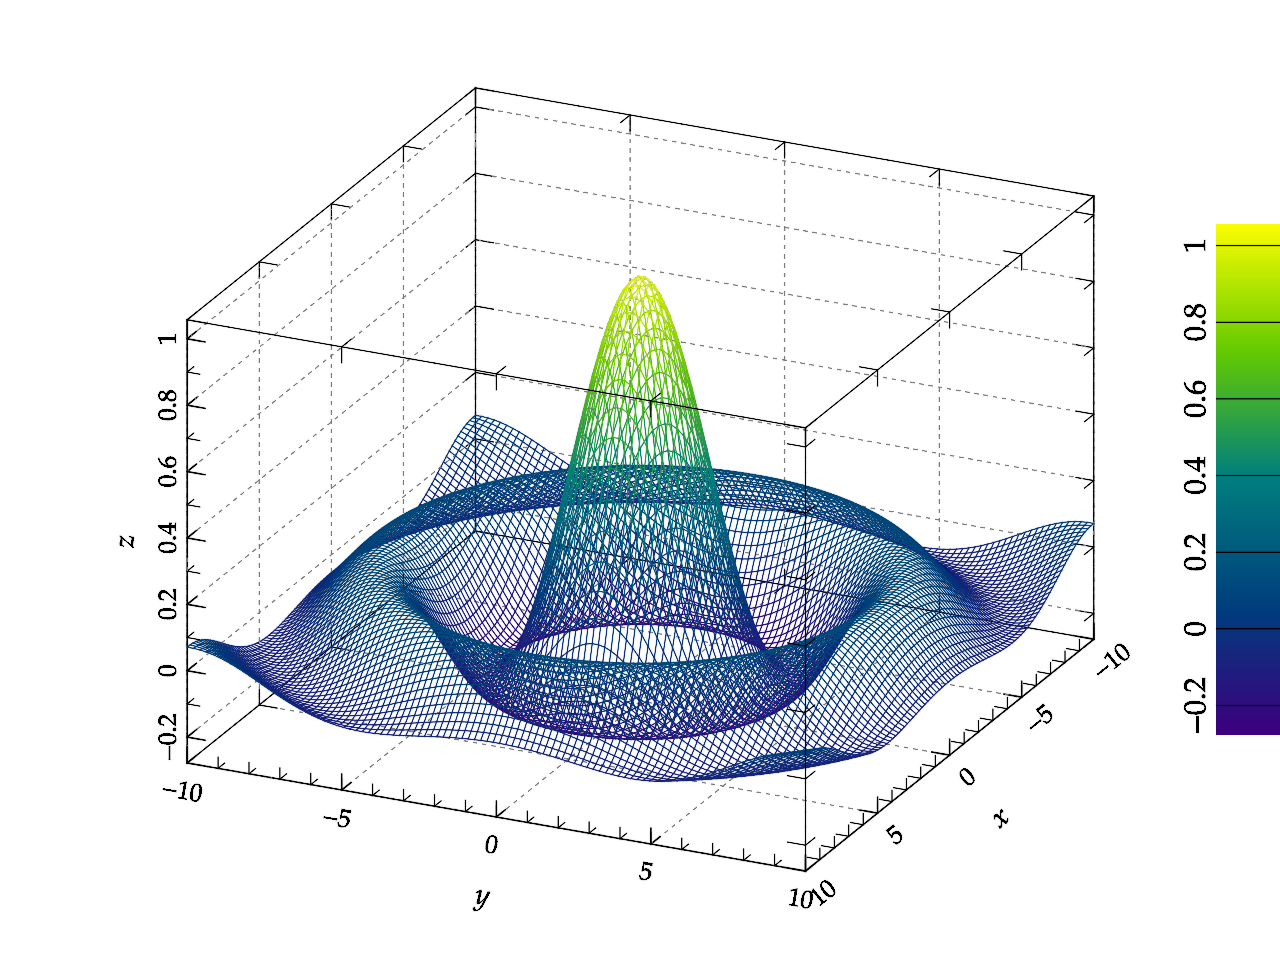
\includegraphics[width=0.45\textwidth]{_graphics/mesh_0.png}}
					\subfloat[with \texttt{nobox}]{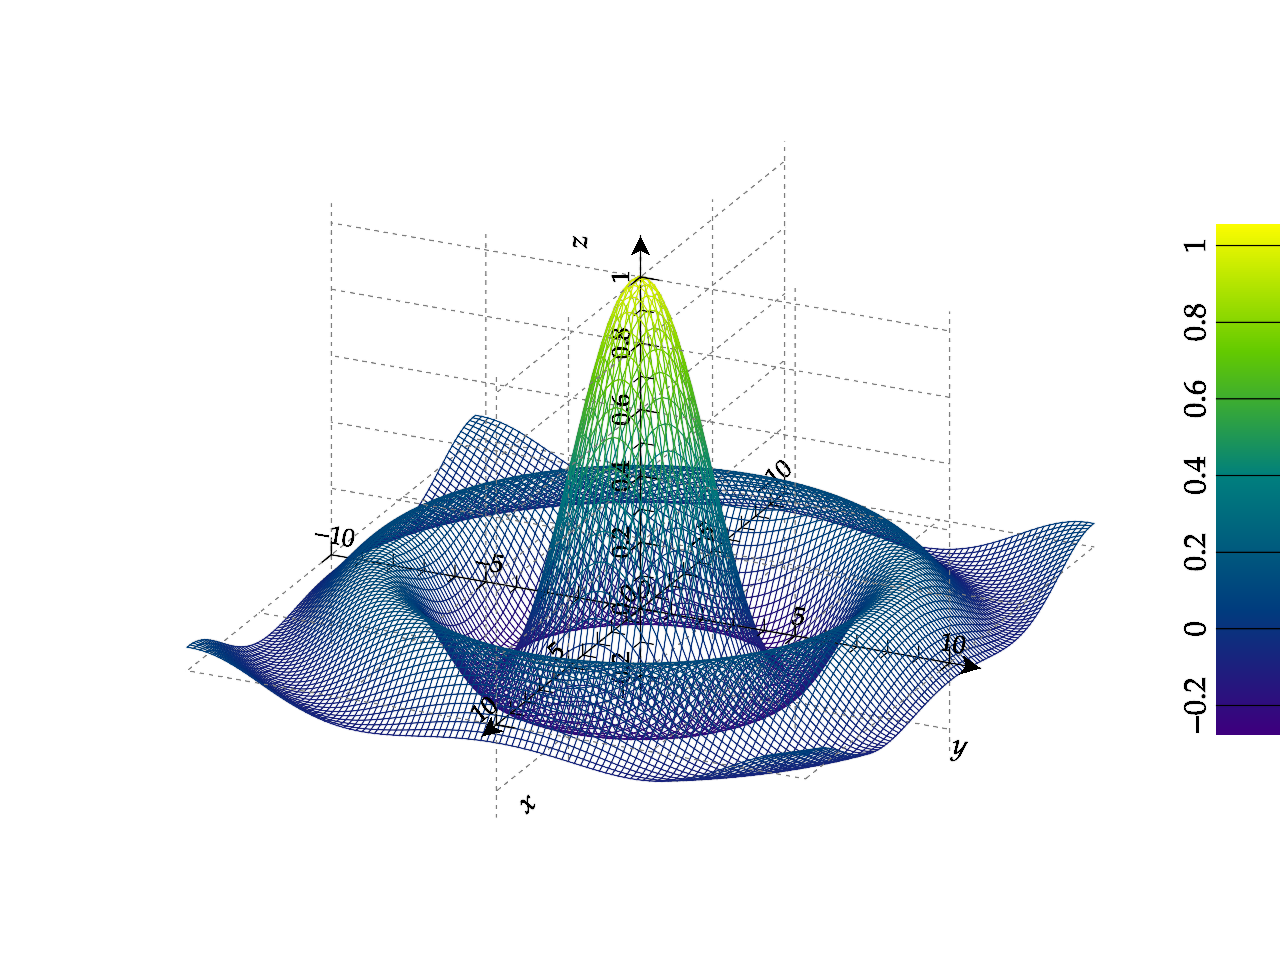
\includegraphics[width=0.45\textwidth]{_graphics/mesh_1.png}}\\
					\subfloat[with \texttt{rotate}]{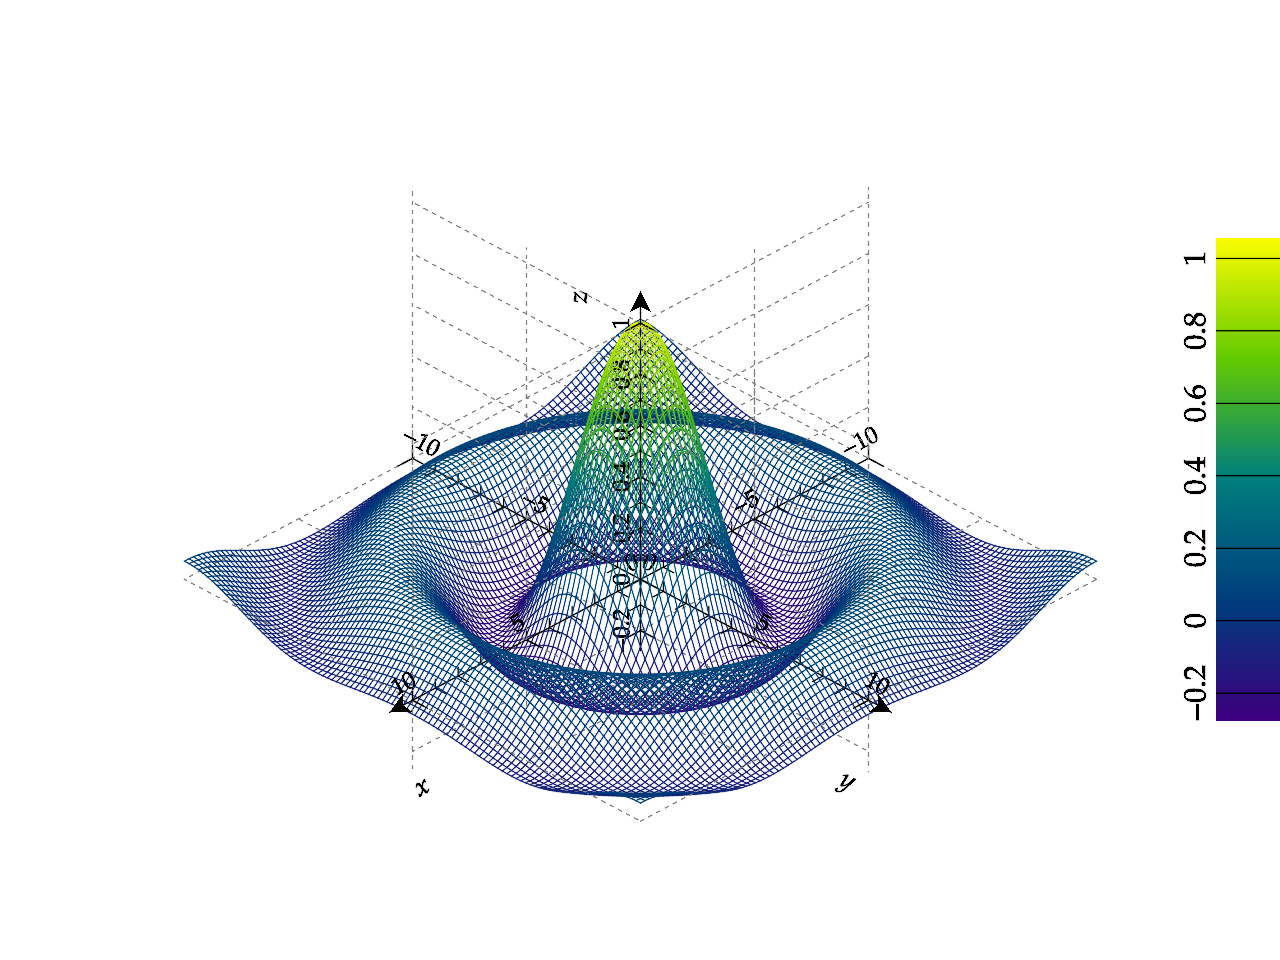
\includegraphics[width=0.45\textwidth]{_graphics/mesh_2.png}}\\
					\subfloat[only \texttt{vect}]{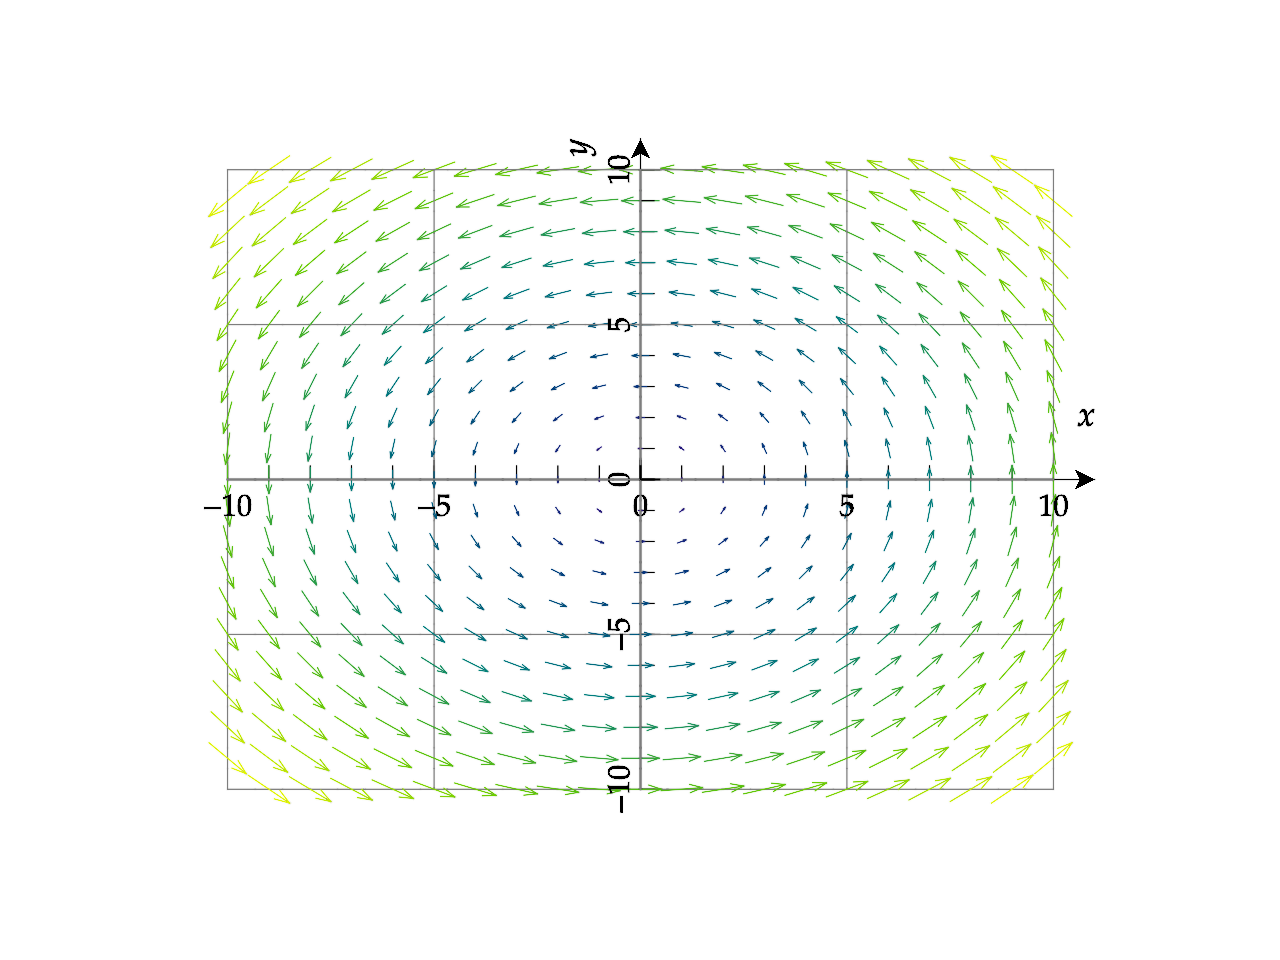
\includegraphics[width=0.45\textwidth]{_graphics/vect_0.png}}
					\subfloat[with \texttt{flength}]{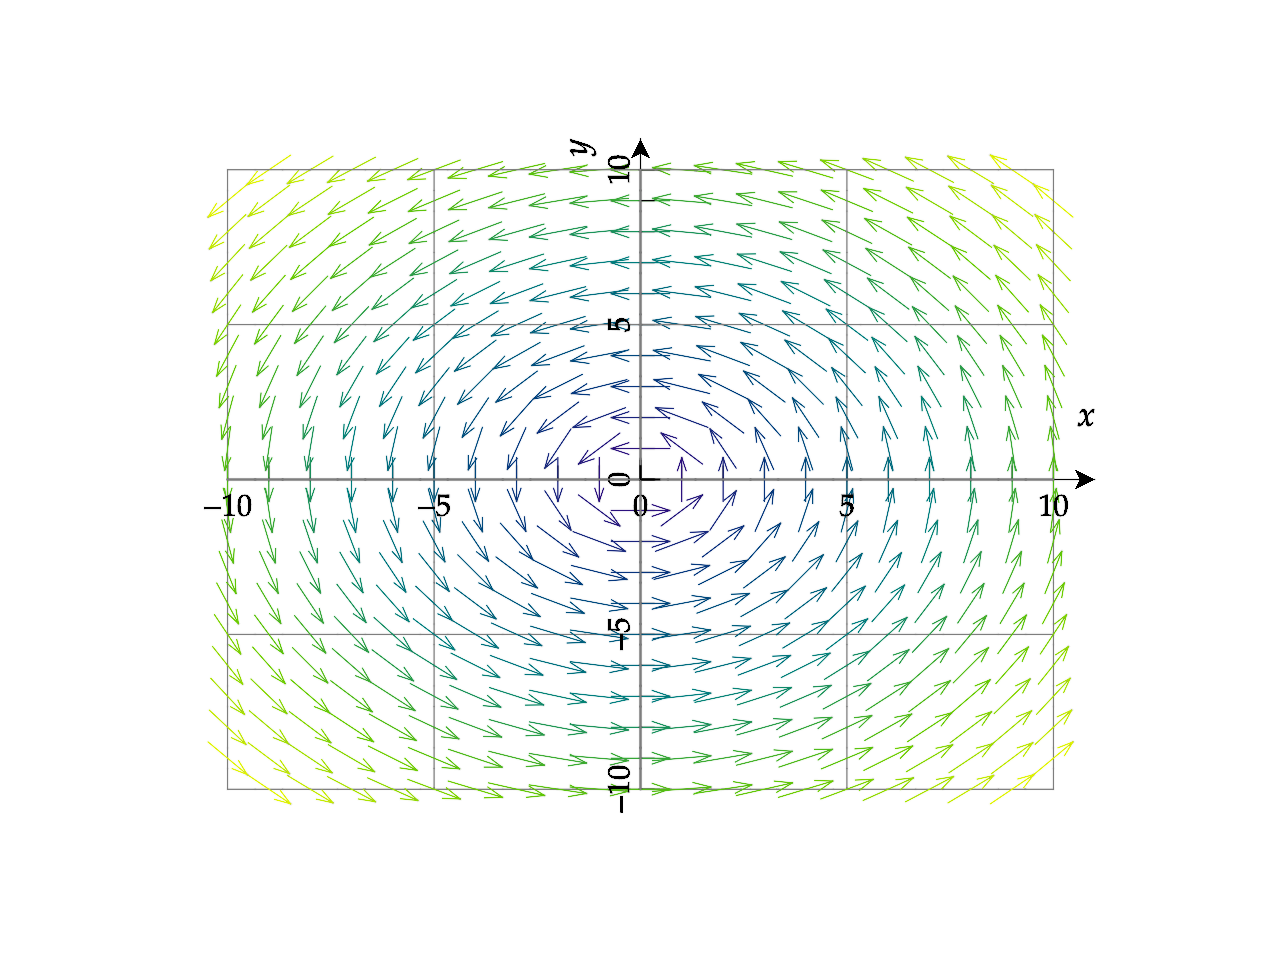
\includegraphics[width=0.45\textwidth]{_graphics/vect_1.png}}
					\caption{Results of the meshgrid and vector plots}
					\label{fig:mesh_vect}
				\end{figure}
				The command \verb+mesh+ creates the desired meshgrid plot (\autoref{fig:mesh_vect}a). The function \verb+norm()+ is the $n$-dimensional, euklidic vector norm (This function will accept an arbitrary number of arguments):
				\begin{equation*}
					\text{norm}(x,y,z,\ldots) := \sqrt{x^2+y^2+z^2+\ldots}
				\end{equation*}
				In this case $\text{norm}(x,y) = \varrho$. Because this was visualized directly after the previous plots in this chapter, you should notice that the meshgrid plot is also surrounded by a box and has a grid in the background. To remove the box, you may enter \verb+nobox+ (\autoref{fig:mesh_vect}b):
				\begin{lstlisting}
mesh sinc(norm(x,y)) -set nobox
				\end{lstlisting}
				
				The meshgrid plot is oriented automatically into a predefined direction. This may also be changed:
				\begin{lstlisting}
mesh sinc(norm(x,y)) -set rotate=45,135
				\end{lstlisting}
				The graph now appears now more tilted and the $x$ and $y$ axes seem to be symmetric to both sides (\autoref{fig:mesh_vect}c). You probably notice that the graph was oriented with these angular values into the direction of the first space diagonal. The angular values of \verb+rotate+ have to be passed in degrees in the order $\vartheta,\varphi$, where $\vartheta$ tilts the graph and $\varphi$ rotates it.
				
				\helpidx{mesh}
				A further example is the vectorfield plot of a two-dimensional rotation field:
				\[\vec A(x,y) = 2\svec{-y\\x}\]
				This is achieved through\cmd{vect}
				\begin{lstlisting}
vect -2*y,2*x
				\end{lstlisting}
				The first function will be interpreted as the amplitude in $\hat e_x$ direction and the second in $\hat e_y$ direction (\autoref{fig:mesh_vect}d). This command will only accept only one vectorfield per plot.
				
				The length of the vector arrows correspond to the local amplitude of the vectorfield. To deactivate this effect, you may pass
				\begin{lstlisting}
vect -2*y,2*x -set flength
				\end{lstlisting}
				(\autoref{fig:mesh_vect}e).
				
				\helpidx{vect}
			\section{Coordinate Systems}
				The last section of this chapter shall focus on the different coordinate systems. \NR\ supports three different coordinate systems: the \emph{cartesian}, the \emph{polar} or \emph{cylindrical} and the \emph{spherical} one.
				\begin{figure}[htb]%
					\centering
					\subfloat[\texttt{plot} with \texttt{coords=polar}]{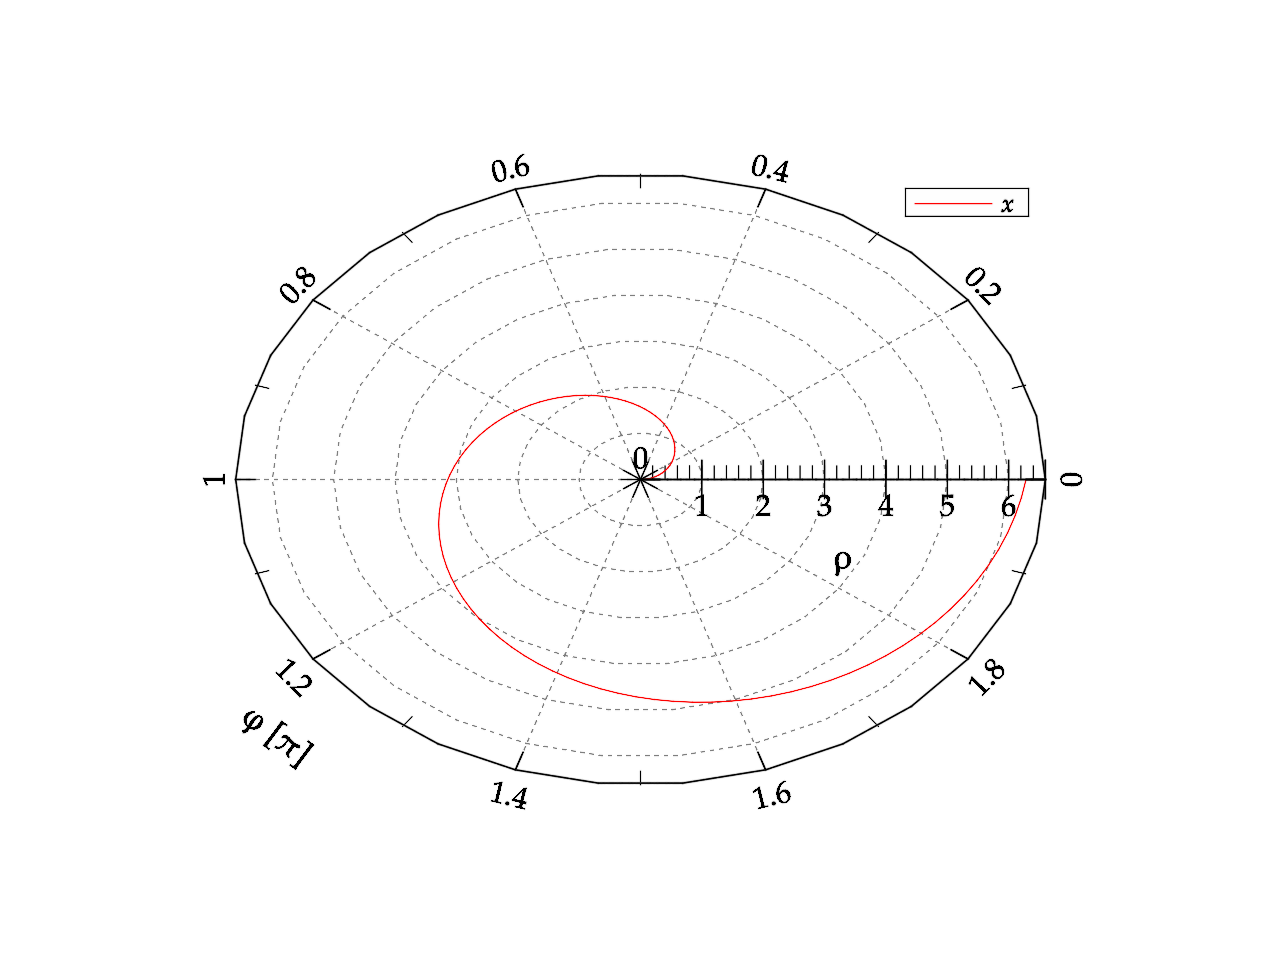
\includegraphics[width=0.45\textwidth]{_graphics/plot_6.png}}
					\subfloat[with larger interval]{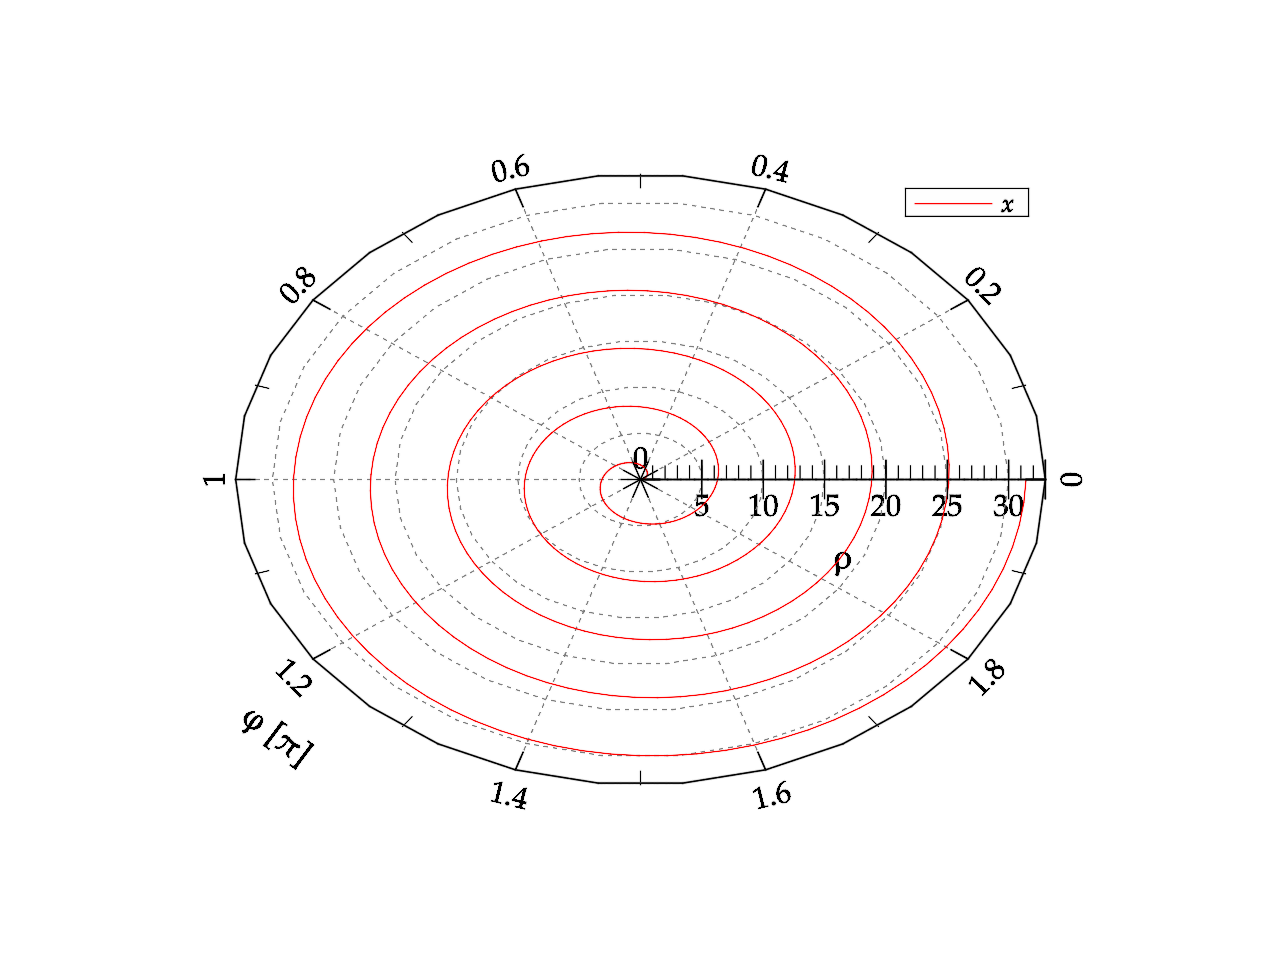
\includegraphics[width=0.45\textwidth]{_graphics/plot_7.png}}\\
					\subfloat[\texttt{surf} with \texttt{light}]{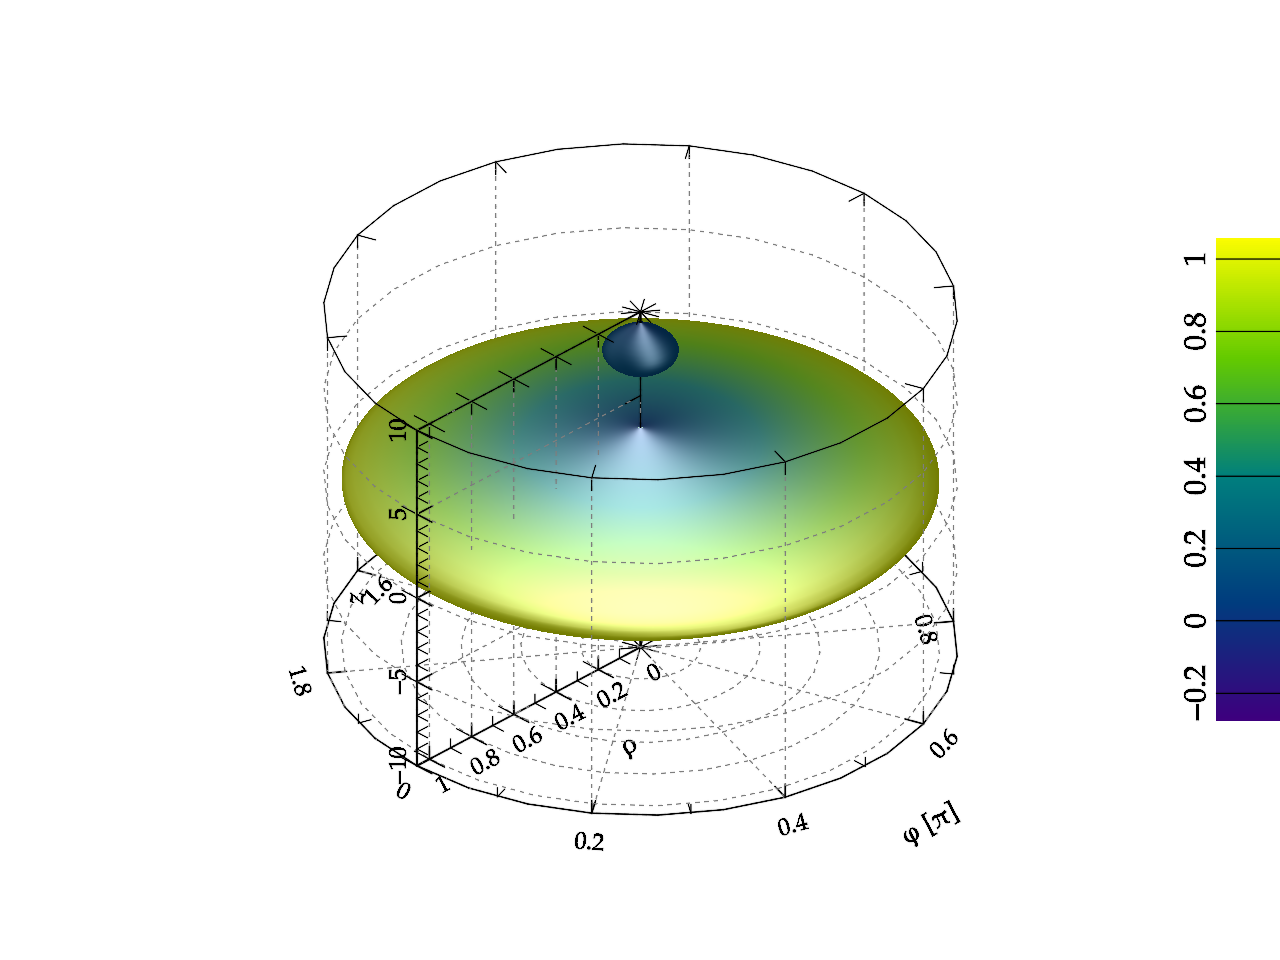
\includegraphics[width=0.45\textwidth]{_graphics/surf_0.png}}
					\subfloat[with \texttt{coords=spherical}]{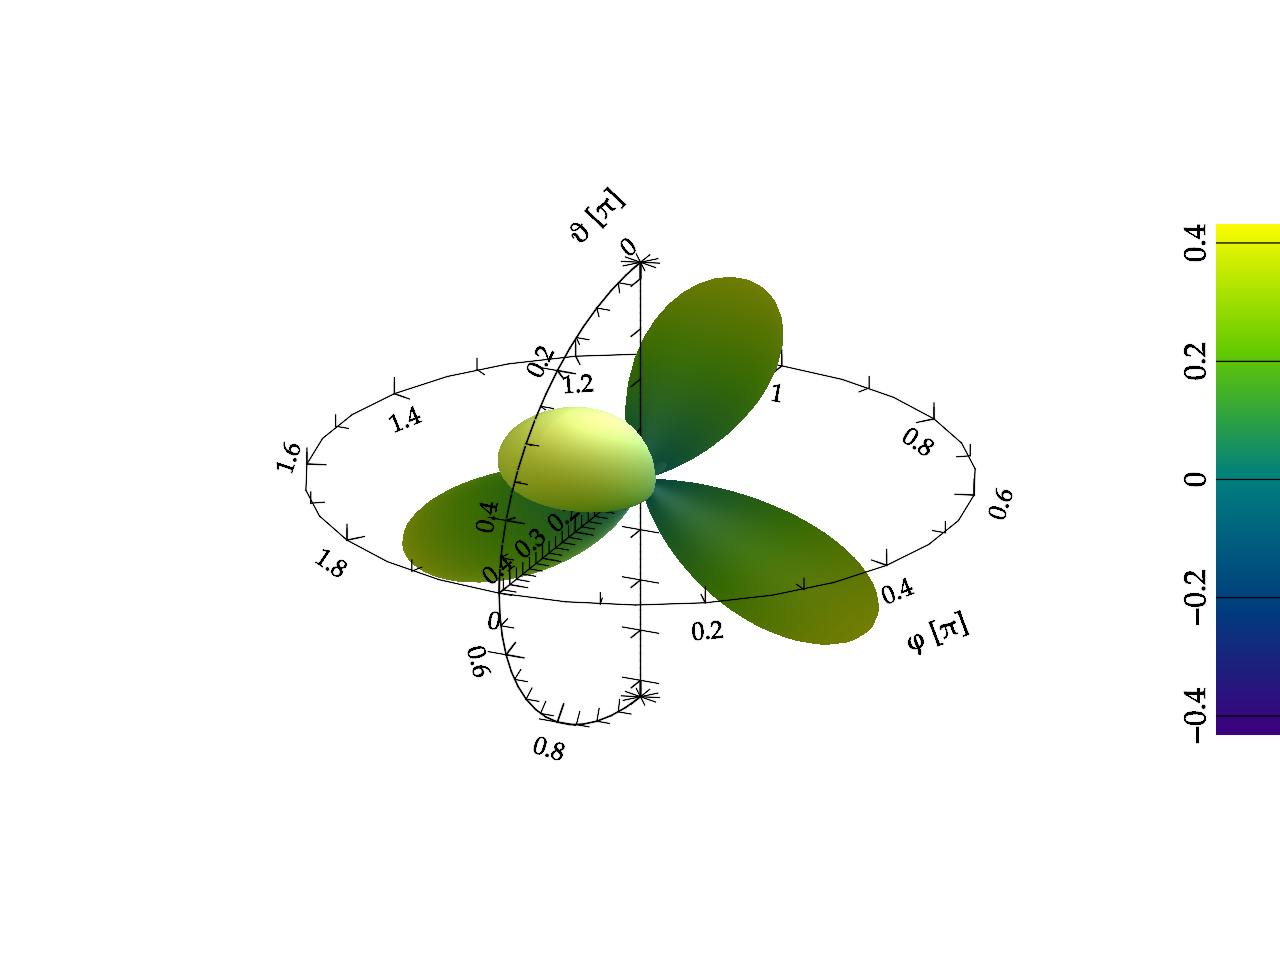
\includegraphics[width=0.45\textwidth]{_graphics/surf_1.png}}
					\caption{Results of the different coordinate systems}
					\label{fig:coords}
				\end{figure}
				
				To change the coordinate system, one uses the option \verb+coords=COORDINATES+. For example: to switch to polar coordinates, one passes the following line (\autoref{fig:coords}a):
				\begin{lstlisting}
plot x -set coords=polar
				\end{lstlisting}
				
				It's noticable that the variable $x$ is used as $\varphi$ and the functions value $y$ as the radial coordinate $\varrho$. The azimuthal axis is displayed in units of $\pi$, but may be changed with the option \verb+axiscale=SCALE+, if desired. 
				
				If one changes the interval for $x$ (meaning $\varphi$), one gets the result of \autoref{fig:coords}b with the following line:
				\begin{lstlisting}
plot x -set coords=polar [0:10*_pi]
				\end{lstlisting}
				It's possible an advantage, to enlarge the number of samples with \verb+samples=WERT+.
				
				In combination with three-dimensional plotting functions, one switches automatically into the cylindrical system, e.g. through
				\begin{lstlisting}
surf sinc(norm(y)) -set light
				\end{lstlisting}
				one gets \autoref{fig:coords}c. The added option \verb+light+ activates the three-dimensional lighting, which emphasises the volume of the plot.
				
				It's getting obvious in this case that the variable $y$ has been used as $z$ and the function value $\Phi(x,y)$ has been interpreted as the radial variable $\varrho$.
				
				Last but not least, the spherical coordinate system shall be presented here. One switches with
				\begin{lstlisting}
surf Y(3,2,y,x) -set coords=spherical
				\end{lstlisting}
				to this system and creates the neat Spherical Harmonics (its real part) $Y_{3\,2}(\vartheta,\varphi)$ in \autoref{fig:coords}d. In this coordinate system $y$ is used as $\vartheta$, $x$ is again $\varphi$ and the function value $\Phi(x,y)$ is presented through the radial coordinate $r$.
				
				\helpidx{coords}
		\chapter{Tables: the Cache}
			\NR\ manages large datasets as tables. As previously mentioned, the default table for loaded data is \verb+data()+. However, this table is \emph{read only}. If you need a table, which you may modify to your needs, you've to use the so-called \emph{caches}.
			\section{Concept}
				Caches are tables in \NR, whose content---similar to usual variables---may be modified freely. Their sizes are arbitrary and fit always to the needs of the user. As default, the default cache \verb+cache()+ already exists. You may also add additional caches.
				
				Caches are autosaving their contents. If the content of a cache is altered, these changes are saved to an external file after the autosave interval is passed. The caches and their contents are automatically recreated after a restart so that you can continue your work immediately.
			\section{Creating and Removing Caches}
				You can use the command \verb+new+ to create new caches (this command may also create further objects):\cmd{new}
				\begin{lstlisting}
new CACHE1(), CACHE2(), CACHE3(), ...
new amplitude(), phase(), results()
				\end{lstlisting}
				You may use the created caches just like the standard \verb+cache()+. If one or more caches of the list are already existing, \NR\ won't change them in any way.
				
				\helpidx{new}
				Custom created caches may also be removed, if their memory is not needed any more for further calculations:\cmd{remove}
				\begin{lstlisting}
remove CACHE1(), CACHE2(), CACHE3(), ...
remove amplitude(), phase(), results()
				\end{lstlisting}
				However, the memory, which is occupied by \NR, is only freed after a restart.
				
				\helpidx{remove}
				You may also rename caches instead of removing them:\cmd{rename}
				\begin{lstlisting}
rename -CACHE1=NEWNAME
rename -amplitude=phase
				\end{lstlisting}
				
				To remove all caches at once and free the complete memory, you may use 
				\begin{lstlisting}
clear cache()
				\end{lstlisting}
				This will also free all the occupied memory of \NR. If you only want to delete the contents of a cache, just use \cmd{delete}
				\begin{lstlisting}
delete CACHE(i1:i2,j1:j2)
				\end{lstlisting}
				
				\helpidx{cache}
			\section{Usage}
				You may use caches similar to the \verb+data()+ table. The central difference is the fact that the contents of caches may be altered. This means, you can also assign new values similar to variables to their elements:\cmd{cache()}
				\begin{lstlisting}
CACHE(:,1) = VALUE1, VALUE2, VALUE3, ...
CACHE(4,5:) = data(:,1)
CACHE(:,1) = CACHE(2,:)
				\end{lstlisting}
				The new values replace the already available values in \verb+CACHE()+.
				
				At all location, where we used \verb+data()+ previously, you may also use caches with the identical syntax. Internally there's no difference (except of the possibility of changing elements) between \verb+data()+ and the caches:
				\begin{lstlisting}
hist cache(:,1)
stats cache()
fit cache(:,4:5) -with=A*sin(B*x+C) params=[A=1, B=1, C=0]
				\end{lstlisting}
				
				Data, which is created by some commands (e.g. \verb+datagrid+), is sometimes written automatically to \verb+cache()+. Also, some of the commands are creating their target caches by themselves.
			\section{Sorting, Smoothing and Resampling}
				Sometimes one has to modify the data points further that one can reasonable process them. \NR\ offers the possibility to sort, smooth or resample (change the number of data points) the data.
				
				The data in a cache (and in principle also in \verb+data()+) may be sorted ascending or descending. In the following one might find distinct thresholds or points of interest in the measured data more easily.
				
				Through entering\cmd{sort}
				\begin{lstlisting}
CACHE -sort
				\end{lstlisting}
				the whole cache \verb+CACHE+ is sorted ascending. To sort it descending, one has to use the value \verb+desc+
				\begin{lstlisting}
CACHE -sort=desc
				\end{lstlisting}
				Using the option \verb+cols+ to columns, which shall be sorted, may be selected. In addition one may select a group of columns, which shall be sorted according an index column (if, for example, $x$ values and their function values are sorted arbitrary, the function values may be sorted according to the $x$ values without losing the connection between the  $x$ values and the function values):
				\begin{lstlisting}
CACHE -sort cols=COLUMNS[COLUMNGROUPS]
cache -sort cols=5[2:4]
				\end{lstlisting}
				
				\helpidx{cache}
				In addition to sorting the data, the data points in a cache may be freed from noise and comparable artifacts. This is achieved through smoothing the data points.
				
				The command\cmd{smooth}
				\begin{lstlisting}
smooth CACHE(i1:i2,j1:j2) -order=ORDER
				\end{lstlisting}
				smooths the cache \verb+CACHE+ in the selected range, where the data points are interpolated linearily over \verb+ORDER+ data points. \NR\ will smooth the data in two dimensions automatically, if this is reasonable according to the selected range. To switch this to column- or linewise smoothing, one may pass the options \verb+lines+ and \verb+cols+.
				
				Smoothing is in principle similar to applying a low-pass filter. If high-frequent data is of interest, smoothing will destroy this information partly or sometimes completely. As a test one might subtract the smoothed from the noisy data and plot the result. If only noise was removed, the plot should only display noise as well.
				
				\helpidx{smooth}
				To alter the number of data points (e.g. if the sample rate is not fitting or one wants to combine different data rows) \NR\ may interpolare further samples into the data or remove them as well.
				
				You'll achieve this with\cmd{resample}
				\begin{lstlisting}
resample CACHE(i1:i2,j1:j2) -samples=SAMPLES
				\end{lstlisting}
				The number of samples is altered columnwise to \verb+SAMPLES+. If \verb+SAMPLES+ is larger than the selected range, no information is lost, because the new data points are interpolated from the previous ones. If the number is smaller, of course information is lost.
				
				\helpidx{resample}
			\section{Statistics Functionalities}
				Caches (and the \verb+data()+ table as well) may execute global statistics operations on the data (similar to \verb+stats+ and statistics functions \verb+std()+, \verb+avg()+, \ldots). One has to use the caches as a command and append the desired statistics function as a parameter (there are no parentheses in the expression in this case):
				\begin{lstlisting}
CACHE -avg
CACHE -std
...
				\end{lstlisting}
				This calculates the average/standard deviation/etc. of the whole table as a single value. The additional options may be restricted further: the option \verb+grid+ calculates the statistics and considers the cache as a datagrid. The option \verb+cols+ calculates the values column- and \verb+lines+ linewise. The options \verb+lines+ and \verb+cols+ may be combined with \verb+grid+.
		\chapter{NumeRe Scripts}
			\NR\ scripts provide the possibility to outsource complex calculations and repeated analyses into a file, from where they may be easily and repeatedly executed.
			\section{Concept}
				The concept building the basis for \NR\ scripts is quite easy: all entries, which one might enter into the \NR\ console, are typed into a textfile instead, which will be read by \NR\ afterwards. \NR\ will execute the expressions and commands in the corresponding order and evaluate them.
				
				The advantage is obvious: the order of commands may easily be repeated and errors may corrected fastly without having to retype erverything.
				\paragraph{Note}
					We will talk about \NR\ procedures in a later chapter. These represent the programmability of \NR. However, most problems, which do not need too complex abstractions, may be solved using \NR\ scripts.
				
				\helpidx{script}
			\section{Syntax Highlighting}
				The syntax of \NR\ scripts is highlighted automatically, if the file was saved with the extension >>.nscr<<. It's a central part of the \NR\ editor. It provides highlighting of syntax elements, of matching parentheses and control flow blocks (e.g. \verb+if ... else ... endif+).
				
				Everybody is free to change the colours of the syntax highlighting to his or her need. This may be done in the options dialogue, which is available in the tools menu, at the tab >>Style<<. 
			\section{A Simple Script}
				As example, a simple script is presented here.
				
				To create a \NR\ script fast and easily, one uses the corresponding item in the file menu or click on the tool in the toolbar or enter 
				\begin{lstlisting}
new -script=first
				\end{lstlisting}
				into the \NR\ console. A \NR\ script with the name >>first.nscr<< is created in \verb+<scriptpath>+, which is in the first two cases opened automatically in the editor. In the latter case the line\cmd{edit}
				\begin{lstlisting}
edit first.nscr
				\end{lstlisting}
				opens the \NR\ script in the \NR\ editor so that it may be edited. (The file extension is here necessary, because \verb+edit+ would look for the script in the wrong directory.) Between the both text blocks in the script (everything between \verb+#*...*#+ is a comment and won't be evaluated by \NR) one enters the following lines:
				\begin{lstlisting}
#* Delete the contents of the cache completely *#
delete cache() -ignore

#* Create random numbers *#
random -lines=1e5 cols=2 distrib=uniform mean=0.5 width=1

#* Are the number inside of the circle of unity? *#
cache(:,3) = (cache(:,1)^2+cache(:,2)^2) <= 1 ? true : false;

#* Calculate pi *#
4*sum(cache(:,3))/1e5
				\end{lstlisting}
				where \verb+##+ starts a line comment, which is ignored by \NR, too. The option \verb+ignore+ in the second line suppresses the confirmation, if one is sure that the contents of the cache shall be deleted. \cmd{random}\verb+random+ creates random numbers and writes them into the cache. In this case, two times 100,000 equally distributed random numbers are created in the interval $[0;1]$.
				
				The third expression is the trickiest. Here the result of a condition is written to the third column of \verb+cache()+. If written with words, this means something like
				\begin{quotation}
					\noindent\emph{>>If the length of the vector is smaller or equal to 1, then write >>true<<, otherwise write >>false<< to the cache.<<}
				\end{quotation}
				The so-called \emph{ternary} operator
				\begin{lstlisting}
CONDITION ? TRUE_VALUE : FALSE_VALUE
				\end{lstlisting}\cmd{()? \ldots\ : \ldots}
				is an abbreviation for the \verb+if...else...endif+ fork, which is explained in a later chapter. The advantage of the \emph{ternary} is that it may be executed faster but it cannot contain commands. A list of all possible logical expressions is obtained through
				\begin{lstlisting}
list -logic
				\end{lstlisting}
				At the end of this line one finds a semicolon \verb+;+. This suppresses the output of its result to the \NR\ console.
				
				The whole \NR\ script is a really simple \emph{Monte-Carlo} simulation. Points are placed arbitrary into a square of the length 1 and afterwards it's counted, how many of them are located in the circle of unity, which is part of this square. Assuming that the probability for each point in the square is equal, the relation of the number of all points to the number of points in the circle of unity has to be equal to $\pi/4$.
				
				If one executes the \NR\ script by clicking on >>Execute<< or through\cmd{start}
				\begin{lstlisting}
start first
				\end{lstlisting}
				(the evaluation of \verb+random+ takes a moment), one gets results similar to
				\begin{lstlisting}
3.1364
3.13668
3.1454
3.13952
...
				\end{lstlisting}
				These numbers are quite near to $\pi$, although they are created through a smart usage of random numbers.
				
				If one enlarges the number of random numbers (e.g. \verb+1e6+ instead of \verb+1e5+) the approximation gets even more precise. However, the cache doesn't support an arbitrary number of elements. For even larger numbers one has to use other ways of calculating.
	\part{Advanced Usage}
		\chapter{Definition of Custom Functions}
			\NR\ already contains a large number of predefined functions (see \verb+list -func+). However, it's sometimes useful and practicable, if one may define his own functions, which are e.g. combining already existing ones. \NR\ may store up to 100 custom defined functions.
			\section{Definition}
				\cmd{define}A custom function is defined using
				\begin{lstlisting}
define my_function(ARGS) := EXPRESSION(ARGS)
				\end{lstlisting}
				This line creates the function \verb+my_function()+, which combines the complex expression of the arguments. The names and the number of arguments may be chosen arbitrary, as long as the number of arguments is not larger than 10. If the last argument of the function is called >>\verb+...+<<, one may pass from one to an arbitrary number of values for this argument. You have to ensure that the defined expression is able to handle an arbitrary number of values, e.g.:\cmd{"\ldots"\:}
				\begin{lstlisting}
define my_function(x,...) := x*sum(...)
				\end{lstlisting}
				
				The name of the function may be chosen freely, while ensuring that it doesn't start with a number nor is identical to a (pre-)defined function.
				
				\cmd{redefine}With
				\begin{lstlisting}
redefine my_function(ARGS) := NEW_EXPRESSION(ARGS)
				\end{lstlisting}
				the function \verb+my_function()+ may be redefined. The number of arguments of course doesn't have to be identical to the previous definition.
				
				Custom defined functions may be supported by comments, which illustrate, what the purpose of the function is. This comment is displayed together with the definition at
				\begin{lstlisting}
list -define
				\end{lstlisting}
				
				The comment may be added to the definition with´
				\begin{lstlisting}
define my_function(ARGS) := EXPRESSION(ARGS) -set comment="COMMENT"
				\end{lstlisting}
				or passed later with \verb+redefine+.
				
				\helpidx{define}
				\cmd{undefine}To remove custom defined functions, you may use the command
				\begin{lstlisting}
undefine my_function()
				\end{lstlisting}
				However, the function storage is cleared at the end of the application automatically. If one wants to prevent this behavior, one may either enter
				\begin{lstlisting}
define -save
				\end{lstlisting}
				and the follwing line after the restart
				\begin{lstlisting}
define -load
				\end{lstlisting}
				to load the functions, or one activate the automatic definition management through
				\begin{lstlisting}
set -defcontrol=true
				\end{lstlisting}
				
				\helpidx{set}
			\section{Conditioned Definition}
				In \NR\ scripts it may be an advantage, if \NR\ won't always raise an error that a function, which shall be defined in that script, is already existing. One possible solution for this case is using the command \verb+redefine+, another is using\cmd{ifndefined}
				\begin{lstlisting}
ifndefined my_function(ARGS) := ...
				\end{lstlisting}
				instead. The function is now only defined, if it isn't already available in the function storage.
			\section{Usage}
				A custom defined function may be used just like the predefined functions, because it is transformed in its definition internally before its execution. Therefore the calls to
				\begin{lstlisting}
my_function(1,2,3)
				\end{lstlisting}
				and 
				\begin{lstlisting}
sin(1)+cos(2)+sinc(3)
				\end{lstlisting}
				are identical for the definition
				\begin{lstlisting}
define my_function(x,y,z) := sin(x)+cos(y)+sinc(z)
				\end{lstlisting}
				You may also pass a lesser number of values as the function has arguments. \NR\ will replace the missing ones automatically with \verb+0+.
		\chapter{Character Strings}
			\NR\ may handle character string in addition to numerical values. First introduced to format the column titles of the tables, character strings are now a major and elaborate part or \NR's architecture.
			\section{Concept}
				Character strings (\emph{strings} for short) are successive chains of characters, which are not interpreted as variables or numerical values by \NR. To achieve this, strings have to be entered as enclosing quotation marks:
				\begin{lstlisting}
"This is a string."
				\end{lstlisting}
				The actual content of the string are all characters between the quotation marks. As a consequence, the string \verb+""+ is empty and has the length 0.
				
				Strings may be modified by special functions: there are functions for converting upper- to lowercase letters (or the other way around), for searching strings inside of strings, to extract a string from another string, to replace strings inside of another one, etc. The main advantage of character strings is the possibility, to format the output and to automate the processing of many files (and they are a precondition for the programming with \NR\ procedures).
				
				\helpidx{string}
			\section{Variable Type}
				The variable type for strings is the third variable type (next to numericals and tables) in \NR. Numerical variables may neiter be converted to string variables nor the other way around. However, there values may (see below).
				
				\NR\ recognizes new string variables automatically using the declaration. This declaration has to be---in contrast to numerical variables, which may be done \emph{on-the-fly}---\emph{always} be followed by a string value (at least an empty string):
				\begin{lstlisting}
numerical_variable = 3.1415926
also_numerical
string = "Hello World!"
also_string = ""
				\end{lstlisting}
				A declaration with the return value of a string function is also possible.
				
				In addition to the string variables, \NR\ knows the \cmd{string()}\verb+string()+ object. This is in principle a single column table, which may contain an arbitrary number of strings. The interval syntax may be used in the argument parentheses to extract a range of strings or a single value. If the argument parentheses are kept empty, the last written string is used automatically.
				
				\helpidx{string}
				Using strings one may modify the column heads of \verb+data()+ and the caches. This is achieved through entering\cmd{data(\#,:)\\cache(\#,:)}
				\begin{lstlisting}
data(#,1) = "Column heading 1"
cache(#,:) = "Column 1", "Column 2", "Column 3"
				\end{lstlisting}
				As you can see, you may use the interval syntax in this context, too. The hash sign \verb+#+ references the column headings.
				
				\helpidx{cache}
			\section{Conversion}
				The value of a string variable may be transformed to a numerical value and the other way around. The content of a string will be interpreted as a new variable, as an expression or even as a command, if applicable. Two functions exist for this purpose:
				\begin{lstlisting}
to_value()
to_cmd()
				\end{lstlisting}
				The function \verb+to_value()+ converts the passed string to a ma\-the\-ma\-tic\-al-nu\-me\-ri\-cal expression and evaluates it correspondingly. \verb+to_cmd()+ transforms the string directly to a command expression.
				
				The inverted conversion may be done in different ways:\cmd{\#VAR\\\#(EXPRESSION)}
				\begin{lstlisting}
#VAR
#(EXPRESSION)
valtostr(EXPR,C,N)
to_string()
string_cast()
				\end{lstlisting}
				The syntax \verb+#VAR+ or \verb+#(EXPRESSION)+ evaluates the following expression/variable and transforms the numerical value directly to a string. Between \verb+#+ and the expression one or more \verb+~+ may be inserted, which will add zeros in front of the value until the corresponding number of characters plus one for the \verb+#+ is reached. The function \verb+valtostr()+ is doing similar, although it's more versatile, because one may pass the filling character through the character \verb+C+.The function \verb+to_string()+ transforms everything, which isn't a string, directly to a string without evaluating it and \verb+string_cast()+ transforms even string variable names into strings.
		\chapter{Loops and Forks as Control Flow Statements}
			The evaluation of \NR\ scripts (and the in one of the following chapters introduced \NR\ procedures) may sometimes be simplified drastically by introducing loops and forks. (However, loops and forks are also usable directly from the \NR\ console.)
			\section{Forks}
				A fork is a location in a script, where the further evaluation of the script depends on the evaluation of a condition. Such forks are represented through the following construct:\cmd{if ()\\\ldots\\elseif ()\\\ldots\\else\\\ldots\\endif}
				\begin{lstlisting}
if (CONDITION1)
	EXECUTE, IF TRUE
elseif (CONDITION2)
	EXECUTE, IF CONDITION1 IS FALSE AND CONDITION2 IS TRUE
else
	EXECUTE, IF ALL CONDITIONS ARE FALSE
endif
				\end{lstlisting}
				
				A fork has to be composed at least out of a \verb+if ()+ and a closing \verb+endif+. In between an arbitrary number of \verb+elseif ()+ and at most one \verb+else+ as \emph{fallback case} may be used, where the \verb+else+ case has to be the last case before the closing \verb+endif+. A fork, which is only composed out of a \verb+if ()+ and a \verb+endif+, will only be executed, if the condition evaluates to true, otherwise it is ignored completely.
			
				The blocks between \verb+if ()+, \verb+endif+ and the other keywords may contain an arbitrary number of commands and expressions. In addition, these blocks may contain further loops and forks.
				
				\helpidx{if}
			\section{Conditioned Loops}
				\cmd{while ()\\\ldots\\endwhile}A conditioned loops will only be executed, as long as the condition evaluates to true. The syntax is as follows
				\begin{lstlisting}
while (CONDITION)
	EXECUTE, AS LONG AS TRUE
endwhile
				\end{lstlisting}
				In the contained block commands and/or expressions or even further loops and forks may be used.
				
				\helpidx{while}
			\section{Counting Loops}
				The execution of a counting loop depends on the value of a index variable. Using the interval syntax, a starting and an ending value have to be passed. If the ending value is \emph{smaller} than the starting value, the counting loop will count backwards automatically. After each single loop pass the index value is increased (or decreased, if the loop counts backwards) by one automatically. The index can be used in the execution block of the loop as a usual variable.
				
				The syntax of a counting loop is as follows:
				\cmd{for ()\\\ldots\\endfor}\begin{lstlisting}
for (INDEX = START:END)
	EXECUTE, AS LONG AS INDEX IS IN [START;END]
endfor
				\end{lstlisting}
				Similar to the other control flow statements, one may use commands, expressions and even further loops and forks in the execution block. After the termination of the counting loop, the index variable will be deleted automatically, if it didn't already exist before the loop.
				
				\helpidx{for}
			\section{Further Control Flow Statements}
				You may influence the execution of a loop with the both commands\cmd{continue\\break}
				\begin{lstlisting}
continue
break
				\end{lstlisting}
				\verb+continue+ jumps over the remaining part of the current execution block and starts a new loop pass. The command \verb+break+ cancels the loop completely and jumps the surrounding execution block. If the surrounding execution block is outside of any loop or fork, the whole loop or fork is terminated. A reasonable application of these commands is using them in the execution block of a fork.
				
				\helpidx{if}
		\chapter{Matrix-Operationen}
			\NR\ ist in Form einer Tabellenkalkulation ausgelegt, da es in der Wissenschaft ungemein wahrscheinlicher ist, dass Messreihen verarbeitet werden müssen, als dass eine Matrix-Operation durchgeführt werden muss. Dennoch ist auch \NR\ in der Lage, mit Matrizen umzugehen und wesentliche Auswertungen durchzuführen.
			\section{Ausführen einer Matrix-Operation}
				Matrix-Operationen verbergen sich hinter dem \verb+matop+- bzw. \verb+mtrxop+-Kommando (Synonyme)\cmd{matop}. Dieses Kommando leitet einen Ausdruck ein, der mittels Matrix-Operationen verarbeitet werden soll, wobei die Matrizen durch Ausschnitte des Caches, eines Datenfiles oder durch spezielle Funktionen repräsentiert werden. Hierbei ist jedoch noch zu beachten, dass alle Auswertungen (also auch die Multiplikation zweier Matrizen) standardmäßig elementweise durchgeführt werden.
				\begin{lstlisting}
matop CACHE(i1:i2,j1:j2) * DATA(i1:i2,j1:j2) + CACHE(:,:) / ...
				\end{lstlisting}
				
				Um eine Matrix-Matrix- oder Matrix-Vektor-Multiplikation durchzuführen, muss der \cmd{... ** ...}\verb+**+-O\-pe\-ra\-tor verwendet werden. Dieser Operator hat eine höhere Priorität als alle anderen Operatoren, daher ist es ggf. wichtig, entsprechend zu klammern. Außerdem ist es wichtig, dass die Dimensionen der Matrizen gemäß den Regeln der Matrizenmultiplikation übereinstimmen.
				\begin{lstlisting}
matop CACHE() ** (DATA() * CACHE())
				\end{lstlisting}
				
				Wenn \verb+matop+ kein Zielcache, in den die Matrix gespeichert werden kann, vorgegeben wird, wird automatisch \verb+matrix()+ verwendet. In diesem Fall werden die Inhalte von \verb+matrix()+ komplett überschrieben.
				
				\helpidx{matop}
			\section{Spezielle Funktionen}
				Spezielle oder temporäre Matrizen bzw. weitergehende Matrix-Operationen können mit den folgenden Funktionen erreicht werden, wenn sie innerhalb des \verb+matop+-Kommandos verwendet werden.
				\begin{itemize}
					\item \verb+cross(MAT)+ berechnet das $n$-dimensionale Kreuzprodukt der $n\times(n-1)$-Matrix \verb+MAT+.
					\item \verb+det(MAT)+ berechnet die Determinante der quadratischen Matrix \verb+MAT+.
					\item \verb+diag(x,y,z,...)+ erzeugt eine Diagonalmatrix mit \verb+x,y,z,...+ auf der Hauptdiagonalen.
					\item \verb+diagonalize(MAT)+ diagonalisiert die quadratische Matrix \verb+MAT+. Sollten die berechneten Diagonalelemente komplex sein, wird eine $n\times2\,n$-Matrix zurückgegeben mit den Realteilen auf der unteren und den Imaginärteilen auf der oberen ersten Nebendiagonalen.
					\item \verb+eigenvals(MAT)+ berechnet die Eigenwerte der quadratischen Matrix MAT und gibt diese in Form eines Vektors zurück. Sind die Eigenwerte komplex, werden sie als zweispaltige Matrix zurückgegeben, mit dem Realteil in der ersten und dem Imaginärteil in der zweiten Spalte.
					\item \verb+eigenvects(MAT)+ berechnet die Eigenvektoren der quadratischen Matrix MAT und gibt diese in Form einer Matrix mit den Eigenvektoren als Spalten zurück. Sind die Eigenvektoren komplex, werden sie als $n \times 2\,n$-Matrix zurückgegeben, mit den Realteilen in den ungeraden und den Imaginärteilen der Vektorkomponenten in den geraden Spalten.
					\item \verb+identity(n)+ generiert eine $n\times n$-Einheitsmatrix
					\item \verb+invert(MAT)+ invertiert die symmetrische Matrix \verb+MAT+, falls eine Inverse existiert.
					\item \verb+matfc(X,Y,Z,...)+ konstruiert eine Matrix aus den Spalten \verb+X,Y,Z,...+. Fehlende Elemente werden durch 0 ergänzt.
					\item \verb+matfcf(X,Y,Z,...)+ konstruiert eine Matrix aus den Spalten \verb+X,Y,Z,...+. Fehlende Elemente werden aus den vorhandenen logisch ergänzt.
					\item \verb+matfl(X,Y,Z,...)+ konstruiert eine Matrix aus den Zeilen \verb+X,Y,Z,...+. Fehlende Elemente werden durch 0 ergänzt.
					\item \verb+matflf(X,Y,Z,...)+ konstruiert eine Matrix aus den Zeilen \verb+X,Y,Z,...+. Fehlende Elemente werden aus den vorhandenen logisch ergänzt.
					\item \verb+one(n,m)+ erzeugt eine $n\times m$-Matrix, die vollständig mit 1-en gefüllt ist. Wird nur eine Dimension vorgegeben, erzeugt \NR\ eine symmetrische Matrix.
					\item \verb+solve(MAT)+ löst das lineare Gleichungssystem, das durch die Matrix \verb+MAT+ beschrieben wird.
					\item \verb+trace(MAT)+ berechnet die Spur der quadratischen Matrix \verb+MAT+.
					\item \verb+transpose(MAT)+ transponiert die Matrix \verb+MAT+ (vertauscht Zeilen mit Spalten).
					\item \verb+zero(n,m)+ erzeugt eine $n\times m$-Matrix, die vollständig mit 0-en gefüllt ist. Wird nur eine Dimension vorgegeben, erzeugt \NR\ eine symmetrische Matrix.
				\end{itemize}
				\begin{lstlisting}
matop matfc({1,2,3},{4,5,6},{7,8,9})
/ 1  4  7 \
| 2  5  8 |
\ 3  6  9 /
matop zero(2,4)
/ 0  0  0  0 \
\ 0  0  0  0 /
				\end{lstlisting}
		\chapter{Spezielle Kommandos}
			An dieser Stelle sollen einige spezielle Kommandos Erwähnung finden, die bisher noch nicht genannt wurden, aber einen großen Teil von \NR's Funktionalität ausmachen.
			\section{Nullstellen}
				\NR\ kann mittels des Kommandos \verb+zeroes+\cmd{zeroes} Nullstellen von Funktionen und Datenreihen suchen. Im Falle von Datenreihen gibt dieses die Indices der Nullstellen (bzw. des Punktes, der sich am nächsten befindet) oder, wenn ein $x$-Datensatz übergeben wurde, den entsprechenden $x$-Wert zurück:
				\begin{lstlisting}
zeroes DATEN()
zeroes DATEN() -set x=XWERTE()
				\end{lstlisting}
				
				Wenn die Nullstellen von Funktionen bzw. der Schnittpunkt zweier Funktionen gesucht werden soll, muss allerdings ein $x$-Intervall vorgegeben werden, in dem \NR\ suchen soll:
				\begin{lstlisting}
zeroes f(x) -set x=x1:x2
				\end{lstlisting}
				
				Im entsprechenden Hilfeartikel finden sich noch weitere Optionen, die \verb+zeroes+ übergeben werden können.
				
				\helpidx{zeroes}
			\section{Extrema}
				Ähnlich wie bei \verb+zeroes+ verhält es sich bei \verb+extrema+.\cmd{extrema} \NR\ kann die Extrema von Funktionen und Datensätzen bestimmen. Bei Funktionen werden die $x$-Werte zurückgegeben, bei Datensätzen die Indices bzw. die $x$-Werte der Punkte, die das Extrema beschreiben.
				\begin{lstlisting}
extrema f(x) -set x=x1:x2
extrema DATEN()
extrema DATEN() -set x=XWERTE()
				\end{lstlisting}
				\paragraph{Anmerkung}Im Gegensatz zu Nullstellen sind Extrema von Datensätzen nicht \emph{wirklich eindeutig} bestimmbar -- zumindest, wenn die Daten mit Rauschen behaftet sind. Dies ist aber in den meisten Fällen erfüllt, daher beschränkt \NR\ sich immer auf die Bestimmung der Indices bzw. $x$-Werte der Maxima bzw. Minima eines Datensatzes anstatt sie, wie bei \verb+zeroes+ ggf. zu interpolieren. Ebenso kann \NR\ aufgrund der numerischen Berechnung Sattelpunkte gar nicht oder nur sehr schlecht identifizieren, da diese Stellen keine Vorzeichenwechsel in der Ableitung aufweisen.
				
				\helpidx{extrema}
			\section{Integration}
				\NR\ kann sowohl Funktionen als auch Daten mittels \verb+integrate+\cmd{integrate} numerisch integrieren, wobei nur für Funktionen eine 2D-Integration unterstützt wird. Ob eine 2D-Integration ausgeführt werden soll, entscheidet \NR\ anhand der übergebenen Integrationsintervalle. Wenn nur ein $x$-Intervall übergeben wird, wird eine 1D-Integration ausgeführt; wenn zusätzlich ein $y$-Intervall übergeben wird, wird zweidimensional integriert.
				
				Mittels des Parameters \verb+-set+ werden das Integrationsintervall und weitere Optionen übergeben, wie z.B. die Präzision der Integration, die Methode, ob die Funktionswerte des Integrals zurückgegeben werden sollen, etc. Details finden sich im entsprechenden Hilfeartikel.
				\begin{lstlisting}
integrate x^2 -set [1:2]
				\end{lstlisting}
				
				Um 1D-Datensätze zu integrieren, sind diese statt der Funktion zu übergeben: wenn nur eine Spalte übergeben wird, wird nur die Summe des Datensatzes berechnet, werden zwei Spalten angegeben, wird die erste als $x$- und die zweite als die entsprechenden $y$-Werte interpretiert und das entsprechende Integral bestimmt.
				\begin{lstlisting}
integrate DATEN(:,1)
integrate DATEN(:,1:3)
				\end{lstlisting}
				
				\helpidx{integrate}
			\section{Ableitung}
				Neben der Integration ist \NR\ auch zur numerischen Ableitung erster Ordnung mittels des Kommandos \verb+diff+\cmd{diff} fähig. Abhängig von den übergebenen Parametern wird dabei die Ableitung an der vorgegebenen $x$-Stelle oder entsprechend der Zahl der gewünschten Stützstellen (\verb+samples+) über ein ganzes Intervall berechnet.
				\begin{lstlisting}
diff sin(x) -set x=1
diff sin(x) -set [0:1]
				\end{lstlisting}
				
				Ebenfalls ist \NR\ in der Lage, Datensätze numerisch zu differenzieren. Wenn hierbei eine Spalte übergeben wird, wird der Abstand zwischen den Stützstellen als 1 angenommen, wenn zwei Spalten angegeben werden, wird die erste als $x$- und die zweite als $y$-Werte interpretiert.
				\begin{lstlisting}
diff DATEN(:,1)
diff DATEN(:,1:2)
				\end{lstlisting}
				Hierbei werden nur die $y$-Werte der Ableitung berechnet. Mittels der Option \verb+xvals+ werden stattdessen die neuen $x$-Werte (die mit den vorgegeben nicht übereinstimmen) bestimmt und zurückgegeben.
				
				\helpidx{diff}
			\section{Taylorentwicklung}
				\NR\ kann mittels \verb+taylor+\cmd{taylor} Funktionen in Abhängigkeit von einer Variablen mittels des Taylor-Verfahrens durch ein Polynom der Ordnung $n \geq 0$ approximieren. Dieses Polynom muss allerdings (außer an der Entwicklungsstelle) nirgends mit der approximierten Funktion übereinstimmen (dies ist eine Eigenschaft der Taylorentwicklung und tatsächlich keine numerische Problematik).
	
				Die Approximation geschieht rein numerisch. Dadurch kommt es zu unvermeidlichen Rundungsfehlern, die für die niedrigen Ordnungen der Entwicklung begrenzt sind. Bis etwa zur Ordnung $n = 10$ (anzugeben durch die Option \verb+n=ORDNUNG+; Standard ist 6) kann \NR\ gute Koeffizienten bestimmen, oberhalb davon kommt es jedoch zu starken Abweichungen im Vergleich zu einer analytischen Berechnung.
				\begin{lstlisting}
taylor cos(x)*exp(-x/2) -set x=2
				\end{lstlisting}
				
				Das entwickelte Polynom wird automatisch als eine Funktion im Funktionenspeicher definiert. Im Allgemeinen wird als Funktionsname \verb+Taylor(x)+ gewählt, wenn allerdings die Option \verb+unique+ übergeben wurde, ist der Funktionsname deutlich komplexer.
				\paragraph{Anmerkung}Bereits existente Funktionen, die mit demselben Namen im Funktionsspeicher vorhanden sind, werden bei dieser Definition überschrieben. Die Option \verb+unique+ generiert jedoch relativ zuverlässig eindeutige Funktionsnamen, da Ausdruck und Ordnung enthalten sind.
				
				\helpidx{taylor}
			\section{Funktionswerte in 1D und 2D} %eval datagrid
				Mittels der Kommandos \verb+eval+ und \verb+datagrid+\cmd{eval\\datagrid} kann \NR\ Funktionswerte von ein- oder zweidimensionalen Funktionen in einem vorgegebenen Intervall und zu einer vorgegebenen Anzahl an Stützstellen auswerten und entsprechend zurückgeben.
				
				Das Kommando \verb+eval+ gibt die Funktionswerte eindimensionaler Funktionen im vorgegebenen Intervall zurück. Dieses Ergebnis kann direkt in einen Cache gespeichert werden. Die Stützstellen werden durch \verb+samples+ vorgegeben (Standard ist 100) und standardmäßig linear verteilt. Durch die Option \verb+logscale+ kann dies auf logarithmische Skalierung geändert werden.
				\begin{lstlisting}
eval FUNCTION(x) -set [x0:x1] OPTIONEN
eval sin(x) -set [0:_2pi] samples=200
				\end{lstlisting}
				
				\helpidx{eval}
				An manchen Stellen erwartet \NR\ sogenannte \emph{Datengitter}. Dies ist ein tabellarischer Datensatz, wobei die $x$-Werte durch die erste, die $y$-Werte durch die zweite und die $z$-Werte durch die darauffolgenden Spalten repräsentiert werden, wobei die Zahl der Zeilen mit der ersten Spalte und die Zahl der Spalten mit der zweiten Spalte übereinstimmen muss.
				
				Diese Datengitter kann \NR\ durch \verb+datagrid+ selbständig erzeugen. Dabei können die Werte für $x$ und $y$ auf verschiedene Weisen gegeben werden: entweder als Intervall in der gemeinsamen Form \verb+[x0:x1,y0:y1]+ oder einzeln durch \verb+x=x0:x1+ oder als Spalte/Zeile eines Datensatzes wie \verb+y=data(:,3)+.
				
				Für $z$ stehen ebenfalls mehrere Möglichkeiten zur Verfügung: entweder als Funktion von $x$ und $y$ ($f(x,y) = \cos(x)\exp(-y)$), als Matrix eines Datensatzes (\verb+cache(3:,7:100)+) oder als einzelne Spalte/Zeile eines Datensatzes (\verb+data(4,2:)+). Im letzteren Fall versucht \NR, die dadurch definierten $(x,y,z)$-Punkte durch Triangulation zu verbinden, und ein Gitter durch lineare Interpolation zu erzeugen.
				\begin{lstlisting}
datagrid z-WERTE -x=x-WERTE y=y-WERTE
datagrid data(:,3) -x=data(:,1) y=data(:,2)
				\end{lstlisting}
				
				Der Parameter \verb+samples=STÜTZSTELLEN+ ist optional und beschreibt nur, wie viele Stützstellen berechnet werden sollen, falls eine Komponente des Datengitters berechnet werden muss. Standardmäßig werden (wie bei den 2D-Plots) $100 \times 100$ Stützstellen berechnet.
				
				Falls die $x$- und $y$-Achse der Datenpunkte vertauscht sind ($x =$ Zeilen, $y =$ Spalten), kann \verb+datagrid+ noch der Parameter \verb+transpose+ übergeben werden. Dadurch werden Zeilen und Spalten beim Erzeugen des Datengitters vertauscht.
	
				Das erzeugte Datengitter wird dabei automatisch an eine freie Stelle im Cache \verb+grid()+ (wird automatisch erzeugt, falls erforderlich) rechts von bereits bestehenden Daten kopiert und kann von dort aus geplottet werden.
				
				\helpidx{datagrid}
			\section{Fouriertransformation}
				Zu den häufig verwendeten Auswertealgorithmen in der modernen Wissenschaft gehören auch Fouriertransformationen, die zum Beispiel auch frequenzabhängige Informationen aus einem vollkommen verrauschten Signal extrahieren können.
				
				\NR\ ist hierzu mit einem Algorithmus zur schnellen Fouriertransformation (\emph{fast fourier transform}) ausgestattet, der durch das Kommando \verb+fft+\cmd{fft} ausgerufen wird und die übergebenen Datensätze zur Analyse in ihre enthaltenen Frequenzen zerlegen kann:
				\begin{lstlisting}
fft DATEN()
				\end{lstlisting}
				Das übergebene Datenobjekt muss mindestens zwei Spalten besitzen: Achsenwerte in der ersten Spalte (Zeit oder Frequenz) und die zugehörige Amplitude in der zweiten Spalte. Werden drei Spalten angegeben, so werden diese als Achsenwerte, Amplitude und Phase (in dieser Reihenfolge) oder -- falls die zusätzliche Option \verb+-complex+ übergeben wird -- als Achsenwerte, Real- und Imaginärteil der Amplitude interpretiert.
				
				\verb+fft+ wird die transformierten Daten als neue Spalten im übergebenen Datenobjekt (bzw. in \verb+cache()+, falls das Datenobjekt \verb+data()+ ist) anlegen. Hierbei wird Frequenz, Amplitude (auch \emph{Magnitude}) und Phase zurückgegeben. Mit der Option \verb+-complex+ werden Real- und Imaginärteile statt Amplitude und Phase zurückgegeben.
				
				Um Daten invers zu transformieren, kann die Option \verb+-inverse+ übergeben werden.
				
				\helpidx{fft}
			\section{Differentialgleichungen}
				Die wenigsten Differentialgleichungen lassen sich analytisch oder durch zufriedenstellende Näherungen lösen. Dies ist das Fachgebiet der Numerik, die die Differentialgleichungen mittels numerischen Algorithmen integriert und dadurch die entsprechenden Trajektorien berechnen kann.
				
				\NR\ bietet einen solchen Integrationsalgorithmus mittels des Kommandos \verb+odesolve+\cmd{odesolve}. Dieser Algorithmus kann Differentialgleichungen erster Ordnung numerisch integrieren. Da man aber auch Differentialgleichungen $n$-ter Ordnung in $n$ Differentialgleichungen erster Ordnung zerlegen kann, stellt dies kein allzu großes Hindernis dar.
				
				Die Differentialgleichung kann dabei aus ein oder mehreren Teilgleichungen bestehen und damit auch ein ganzes System bilden. Die Gleichungen müssen dem folgenden Schema genügen:
				\begin{lstlisting}
dy1/dx = f1(x,y1,y2,...)
dy2/dx = f2(x,y1,y2,...)
...,				
				\end{lstlisting}
				wobei nur die Funktionen \verb+f1()+ bis \verb+fn()+ in dieser Reihenfolge durch Kommata getrennt angegeben werden müssen. \verb+x+ ist hierbei die Integrationsvariable und \verb+y1+ bis \verb+yn+ sind vordefinierte Funktionsvariablen, in denen \NR\ die Ergebnisse des letzten Integrationsschritts ablegt. Alle anderen Variablen werden als Parameter betrachtet.
	
				Differentialgleichungen $n$-ter Ordnung $DGL(x,y,y',y'',\ldots,y^{(n)})$ können stets in ein System von $n$ Differentialgleichungen erster Ordnung überführt werden, indem $n-1$ zusätzliche Funktionen eingeführt werden: $y' = dy1/dx = y2, y'' = dy2/dx = y3, \ldots$ Ein solches System folgt dann dem Schema:
				\begin{lstlisting}
dy1/dx = y2
dy2/dx = y3
...
dyn/dx = DGL(x,y1,y2,...,y(n-1))
				\end{lstlisting}
	
				Die Ergebnisse der Integration werden standardmäßig in den Cache \verb+ode()+ als Tabelle geschrieben. Die erste Spalte enthält dabei die $x$-Werte und die folgenden Spalten die dazu integrierten Funktionswerte.
				
				Um Startwerte vorzugeben (\NR\ wird anderen falls stets 0 verwenden), kann die Option \verb+fx0=STARTWERTE+ verwendet werden. Außerdem kann die Integrationsmethode, die zu verwendenden Toleranzen, die Zahl der berechneten Funktionswerte und andere Dinge modifiziert werden. Details hierzu finden sich in der integrierten Dokumentation.
				\begin{lstlisting}
odesolve DGL(x,y1,y2,...) -set [x0:x1] OPTIONEN
odesolve y2,-sin(y1) -set [0:20] fx0=[0,1]
				\end{lstlisting}
				\paragraph{Anmerkung}\NR\ wird die Zahl der Funktionsvariablen entsprechend der Zahl der Gleichungen bereitstellen: bei einer Gleichung ist nur \verb+y1+ verfügbar, bei zwei \verb+y1+ und \verb+y2+, etc. Werden mehr Variablen benötigt (um z.B. ein vektorielles Problem zu lösen), können 0-Gleichungen als entsprechende Gleichung eingeführt werden, die Variable wird dann jedoch als Konstante betrachtet.
				
				\helpidx{odesolve}
		\chapter{NumeRe-Prozeduren}
			Neben den \NR-Scripten können Befehlsroutinen auch in \NR-Prozeduren ausgelagert werden. Allerdings bieten \NR-Prozeduren deutlich umfassendere Möglichkeiten, Aufgabenstellungen zu abstrahieren. Dazu gehört auch die Möglichkeit, \NR-Prozeduren rekursiv aufzurufen und ihre Rückgabewerte weiter zu verarbeiten.
			\section{Konzept}
				\NR-Prozeduren sind im Prinzip gestaltet wie eine Mischung aus einer selbst definierten Funktion und einem \NR-Script. Zusätzlich dazu kann eine \NR-Prozedur sich auch selbst rekursiv aufrufen (\verb+define+ würde einen Fehler zurückgeben) und deutlich komplexere Befehle und Ausdrücke abarbeiten (Prozeduren sind nicht auf Ausdrücke begrenzt, die sich in einer Zeile ausdrücken lassen müssen).
				
				Mittels \NR-Prozeduren ist es des Weiteren möglich, eigene Unterprogramme in \NR\ zu schreiben oder weitere Funktionalität in Form eines neuen Kommandos hinzuzufügen (dies ist als \emph{Plugin} bekannt).
				
				Der Stellenwert einer \NR-Prozedur innerhalb von \NR\ ist als in etwa das Äquivalent einer Funktion in einer gewöhnlichen Programmiersprache.
				
				\helpidx{procedure}
			\section{Struktur}
				\NR-Prozeduren gliedern sich in ihrer Struktur in drei Teile: Prozedurkopf, Prozedurrumpf und Prozedurfuß. Der Kopf enthält den Namen, die Argumentliste und zusätzliche >>Flags<<, der Prozedurrumpf enthält die kompletten Befehlsroutinen:\cmd{procedure\\\ldots\\endprocedure}
				\begin{lstlisting}
procedure $PROZEDURNAME(ARGLIST) :: FLAGS   ## Prozedurkopf
	PROZEDURRUMPF                           ## Befehle und Ausdruecke
endprocedure                                ## Prozedurfuss
				\end{lstlisting}
				Um eine \NR-Prozedur aufzurufen, gibt man \verb+$PROZEDURNAME(VARS)+ in \NR-Scrip\-ten, anderen \NR-Prozeduren oder der \NR-Konsole an. Die \verb+VARS+ sollten dabei mit der Zahl der Argumente in \verb+ARGLIST+ übereinstimmen. Falls in \verb+ARGLIST+ Defaultwerte für die Argumente angegeben wurden, können diese in \verb+VARS+ auch weggelassen werden. Es werden dann die Defaultwerte für die entsprechenden Argumente verwendet.
				
				Die hier erwähnten >>Flags<< haben auf die gesamte \NR-Prozedur Einfluss und unterbinden oder erlauben bestimmte Verhaltensweise von \NR\ in dieser Prozedur. Im Grunde setzen diese Flags jedoch das Wissen der folgenden Abschnitte und Kapitel voraus:\cmd{explicit\\private\\inline}
				\begin{lstlisting}
explicit
private
inline
				\end{lstlisting}
				Der Flag \verb+explicit+ verhindert die Ausführung von Plugins in dieser Prozedur, \verb+private+-geflagte Prozeduren können nur von Prozeduren desselben Namensraumes aufgerufen werden und Prozeduren mit dem \verb+inline+-Flag erlauben schnellere Schleifenausführungen, wenn die Schleifen nur \NR-Pro\-ze\-du\-ren dieses Typs enthalten. Dafür sind \verb+inline+-Pro\-ze\-du\-ren vergleichsweise eingeschränkt.
				
				Flags können in jeder beliebigen Kombination/Reihenfolge angegeben werden, da sie sich nicht gegenseitig beeinflussen.
				
				Jede \NR-Prozedur muss sich in einer eigenen *.nprc-Datei befinden, die den Namen der Prozedur trägt. Was im ersten Moment jedoch aufwändig und fehleranfällig klingt, kann von voll und ganz von \NR\ erledigt werden. Durch den entsprechenden Menüpunkt im Datei-Menü, durch Klicken auf die Schaltfläche der Toolbar oder durch
				\begin{lstlisting}
new -proc=$PROZEDURNAME
				\end{lstlisting}
				wird die \NR-Prozedur \verb+$PROZEDURNAME+ in \verb+<procpath>/PROZEDURNAME.nprc+ angelegt. Durch die darauffolgende Eingabe von
				\begin{lstlisting}
edit $PROZEDURNAME
				\end{lstlisting}
				kann \verb+$PROZEDURNAME+ im verknüpften Texteditor bearbeitet werden.
				
				Der Prozedurrumpf einer \NR-Prozedur kann im Großen und Ganzen analog zu einem \NR-Script gestaltet sein. Die wesentlichen Besonderheiten werden in den folgende Abschnitten besprochen.
			\section{Lokale und globale Variablen}
				\NR-Prozeduren unterscheiden zwischen lokalen und globalen Variablen. Globale Variablen sind Variablen, die von jeder Prozedur, jedem Script und der \NR-Konsole selbst aufgerufen und verwendet werden können. Demgegenüber sind lokale Variablen, die \emph{nur} in \emph{dieser} Prozedur und auch dann \emph{nur} in \emph{dieser} Rekursion der Prozedur verwendet werden können.
				
				Lokale Variablen werden mittels\cmd{var\\str\\tab}
				\begin{lstlisting}
var VARIABLEN
str ZEICHENKETTENVARIABLEN
tab CACHES
				\end{lstlisting}
				deklariert. Diese Kommandos dürfen je Prozedur nur einmal auftreten und deklarieren jeweils einen Satz an lokalen numerischen Variablen, Zeichenkettenvariablen oder lokalen Caches. Diese Variablen werden am Ende der Prozedur automatisch wieder gelöscht. (Lokale Variablen können genauso wie globale heißen. In einer \NR-Prozedur haben die lokalen Variablen dann die höhere Priorität. Man spricht dann von \emph{schattieren}.)
			\section{Rückgabewerte}
				Standardmäßig geben \NR-Prozeduren den Wert \verb+true+ zurück, wenn die Auswertung die Zeile \verb+endprocedure+ erreicht. \NR-Prozeduren können aber auch andere Werte zurückgeben, wenn\cmd{return}
				\begin{lstlisting}
return WERT
				\end{lstlisting}
				an der entsprechenden Stelle in der Prozedur auftritt. \NR\ wird die Prozedur auf jeden Fall verlassen, sobald \NR\ an einer Stelle auf dieses Kommando trifft (Es kann auch mehrmals in einer Prozedur verwendet werden). \verb+WERT+ kann dabei entweder ein numerischer Wert oder eine Zeichenkette sein. Davon abgesehen kann auch explizit \verb+true+ oder \verb+false+ als \verb+WERT+ verwendet werden.
				
				Dabei muss \verb+WERT+ nicht auf einen einzigen Wert beschränkt werden. Es können auch mehrere numerische Werte oder mehrere Zeichenketten zugleich zurückgegeben werden. Sogar die Kombination aus beiden Variablentypen ist möglich, aber zugleich auch fehleranfälliger als Werte eines einzelnen Variablentyps, da die ggf. aufrufende Prozedur auch mit dem Satz an Werten zurecht kommen muss.
				
				Werden Prozeduren mit mehreren Rückgabewerten für \verb+while+-Schleifen- oder \verb+if+-Bedingungen verwendet, so wird dort nur der erste Wert für die Logikoperationen ausgewertet.
				
				Der spezielle Wert \verb+void+ dient dazu, \NR\ mitzuteilen, dass diese Prozedur tatsächlich \emph{keinen} Rückgabewert hat.
			\section{Namensräume}
				Ähnlich wie C++ ist \NR\ mit Namensräumen ausgestattet, die es erlauben, Prozeduren gleichen Namens aber unterschiedlichen Verhaltens in unterschiedlichen Namensräumen zu besitzen. Aufgerufen werden Prozeduren aus einem anderen als dem Standardnamensraum \verb+main+ durch 
				\begin{lstlisting}
$NAMENSRAUM~PROZEDURNAME(VARS)
				\end{lstlisting}
				Die entsprechende Prozedur \verb+$PROZEDURNAME+ liegt dabei in der Datei 
				\begin{lstlisting}
<procpath>/NAMENSRAUM/PROZEDURNAME.nscr
				\end{lstlisting}
				Das Kommando \verb+new+ kann auch automatisch Prozeduren in untergeordneten Namensräumen erzeugen, wenn dies entsprechend angegeben wird:
				\begin{lstlisting}
new -proc=$NAMENSRAUM~PROZEDURNAME
edit $NAMENSRAUM~PROZEDURNAME
				\end{lstlisting}
				Gleiches gilt aber auch, wenn man die Funktionen der graphischen Oberfläche verwendet.
				
				Werden in einer Prozedur häufiger \NR-Prozeduren aus einem bestimmten Namensraum aufgerufen, kann dieser Namensraum auch als temporärer Standardnamensraum vorgegeben werden, indem\cmd{namespace}
				\begin{lstlisting}
namespace NAMENSRAUM
				\end{lstlisting}
				in die Prozedur eingebunden wird. (Prozeduren aus anderen Namensräumen können jedoch immer noch aufgerufen werden, indem der Namensraum wie oben gezeigt explizit angegeben wird.)
			\section{Fehlerbehandlung}
				\NR-Prozeduren verfügen über ein simples Verfahren, mit Fehlern umzugehen. Tritt ein Fehler auf, der auf keine sinnvolle Art behandelt werden kann (z.B. in Form einer falschen Eingabe), dann kann mittels des Kommandos\cmd{throw}
				\begin{lstlisting}
throw
				\end{lstlisting}
				ein unmittelbares Abbrechen der Prozedurauswertung erzwungen werden. Dieses Kommando wird bis ganz oben durchgereicht, bis es schließlich auf die Standard-\NR-Konsole trifft und dort eine entsprechende Fehlermeldung produziert.
				
				Etwas informativer wird die Fehlermeldung durch Übergeben einer eigenen Meldung. Dies geschieht in Form einer Zeichenkette
				\begin{lstlisting}
throw "Das ist die Fehlermeldung."
				\end{lstlisting}
				die in der \NR-Konsole schließlich angezeigt wird.
			\section{Debugging}
				In den wenigsten Fällen wird eine \NR-Prozedur beim ersten Versuch bereits lauffähig und fehlerfrei sein. Hierzu sind kleinere Tipp- oder Logikfehler viel zu wahrscheinlich. Beim Ausführen einer solchen fehlerhaften \NR-Prozedur wird \NR\ ggf. an einer Stelle abbrechen, wenn es sich um einen Syntaxfehler handelt, aber nicht unbedingt, wenn ein Rechenfehler aufgetreten ist.
				\begin{figure}[htb]
					\centering
					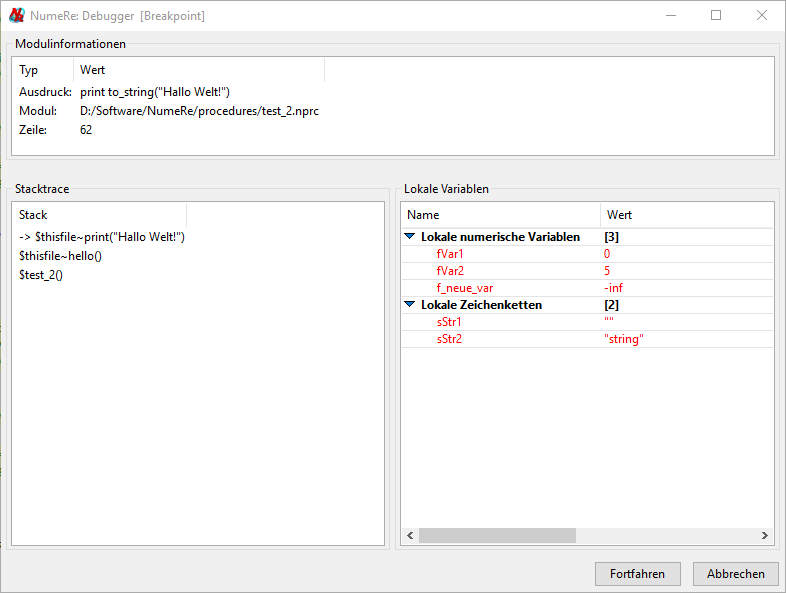
\includegraphics[width=\textwidth]{_graphics/debugger.png}%
					\caption{Der \NR-Debugger an einem Breakpoint. Mit rot werden die Änderungen zum letzten ausgewerteten Breakpoint hervorgehoben}%
					\label{fig:debugger}%
				\end{figure}
				
				\NR\ besitzt zum Aufspüren und Entfernen solcher Fehler einen sogenannten \NR-\emph{Debugger} (\autoref{fig:debugger}). Dieser kann durch den entsprechenden Menüpunkt im Werkzeuge-Menü oder durch Klicken auf die Schaltfläche der Toolbar aktiviert werden und listet bei Syntaxfehlern automatisch den fehlerhaften Ausdruck, die ungefähre Zeile des Ausdrucks, das fehlerhafte Modul (Datei), eine Stacktrace und alle lokalen Variablen der aktuellen Prozedur inklusive ihrer Werte. Mittels der Stacktrace kann rekonstruiert werden, in welcher Prozedur der Fehler aufgetreten ist und welche Argumente an diese übergeben wurden.
				
				Zusätzlich zum automatischen Listen bei Syntaxfehlern kann der \NR-Debugger vergleichbare Informationen an einem \emph{Breakpoint} liefern. Ein temporärer Breakpoint kann durch die Funktionen der Toolbar oder durch Klicken auf die betreffende Zeile der Seitenleiste gesetzt werden. Man beachte, dass in Zeilen, die nur aus Kommentaren bestehen, oder Zeilen, die leer sind, \emph{keine} temporären Breakpoints gesetzt werden können. 
				
				Permanente Breakpoints werden mittels \verb+|>+ am Anfang einer Zeile gesetzt, sind aber selten nötig. \NR\ unterbricht, bevor die \emph{aktuelle Zeile} ausgewertet wird, und listet Stacktrace und Variablenwerte. Durch Klicken auf >>Fortsetzen<< kann die Auswertung fortgesetzt werden, durch >>Abbrechen<< wird die Auswertung komplett abgebrochen. (Außerhalb des Debug-Modus werden Breakpoints selbstverständlich ignoriert.)
				
				\helpidx{debugger}
		\chapter{Animierte Graphen}
			Manchmal kann es hilfreich sein, wenn man den zeitlichen Verlauf einer Größe mithilfe eines animierten Graphen verdeutlichen kann. \NR\ verfügt über eine fest implementierte Möglichkeit, eine solche Animation zu erzeugen. Eine Animation kann aber natürlich auch mittels einer Schleife erzeugt werden, indem die Frames einzeln gespeichert und später zu einer Animation zusammengesetzt werden.
			
			Um eine Animation direkt durch \NR\ erzeugen zu lassen, muss mindestens an einer Stelle die Variable \verb+t+ in einem zu plottenden Ausdruck verwendet werden. Diese Variable ist in diesem Fall der Zeitparameter, der für die Animation variiert wird. Zusätzlich muss die Option \verb+animate+ bei einem Plotvorgang übergeben werden:\cmd{animate}
			\begin{lstlisting}
PLOTCMD AUSDRUCK(t,VARS) -set animate OPTIONEN
			\end{lstlisting}
			Dies wird eine Animation erzeugen, die aus mehreren, inkludierten Einzelbildern besteht. Im \NR-GraphViewer kann diese Animation abgespielt oder die Frames einzeln betrachtet werden.
			
			\helpidx{plotoptions}
			\paragraph{Anmerkung}
				\NR\ kann nativ keine Animationen aus Datensätzen erzeugen. Dies ist u.A. der Tatsache geschuldet, dass der Zeitparameter auch nicht-ganzzahlig Werte annehmen kann, Tabellenobjekte allerdings nur ganzzahlige Indices akzeptieren. Um eine Animation aus Datensätzen zu generieren, muss folglich auf die Einzelbilderzeugung mittels einer Schleife zurückgegriffen werden.\bigskip\\
			Standardmäßig erzeugt \NR\ 50 Frames je Animation mit einer jeweiligen Dauer von $1/25$~s und verwendet als Zeitparameter \verb+t+ das Intervall $[0;1]$. Dies kann natürlich geändert werden, allerdings kann es bei zu vielen Frames zu Speicherschwierigkeiten kommen, da die Frames einzeln im Speicher abgelegt werden müssen:
			\begin{lstlisting}
PLOTCMD AUSDRUCK(t,VARS) -set t=0:2 animate=100 OPTIONEN
			\end{lstlisting}
			Nun wird die Animation mit 100 Frames erzeugt, wobei der Zeitparameter das Intervall $[0;2]$ verwendet.
			\paragraph{Anmerkung}
				Manche Plotarten können möglicherweise zu viel Speicherplatz erfordern, so dass eine Animation nicht möglich ist. Es kann hierbei helfen, die \verb+samples+ der Abbildung zu reduzieren.
		\chapter{Zusammengesetzte Graphen}
			Es mag vorkommen, dass ein gewünschtes Plotlayout nur erreichbar ist, wenn man zwei Plotstile miteinander kombinieren könnte. Dies ist in \NR\ auch möglich, wenn man\cmd{compose\\\ldots\\endcompose}
			\begin{lstlisting}
compose
	PLOTSTIL1
	PLOTSTIL2
	...
endcompose
			\end{lstlisting}
			verwendet. Der \verb+compose+-Modus nimmt allerdings nur Plotkommandos auf, das heißt, dass die für die jeweiligen Plotstile nötigen Berechnungen bereits zuvor abgeschlossen sein müssen.
			
			Manche Plotoptionen gelten für einen kompletten zusammengesetzten Plot (wie z.B. Plotintervall, Achsenbeschriftung, Gitter, etc.), andere können je nach Plot aus- oder eingeschaltet werden (z.B. Transparenz, Lichteffekt, zusätzliche Konturlinien, Fehlerbalken, etc.). Die Plotfarben und Linienstile können auch für jeden Plot einzeln gewählt werden, jedoch ist zu beachten, dass \NR\ einen internen Zähler für alle Linien hat und dieser für jeden Plot erhöht wird. Demzufolge müssen die Styleinformationen ggf. entsprechend angepasst werden.
			
			Mithilfe des \verb+compose+-Modus können Plots zwei verschiedener Größen gemeinsam dargestellt werden, z.B. ein Vektorfeld zusammen mit seinem Potential. Es spielt hierbei keine Rolle, in welcher Reihenfolge \verb+vect+ und \verb+dens+ angegeben werden, da \NR\ die Plots intern in eine sinnvolle Reihenfolge bringt:
			\begin{lstlisting}
compose
	dens 1/norm(x,y)
	vect x/norm(x,y)^3,y/norm(x,y)^3
endcompose
			\end{lstlisting}
			
			\helpidx{compose}
			Der \verb+compose+-Modus erlaubt es des Weiteren, die Beschränkung auf eine einzelne Funktion bei den 3D-Plotstilen (außer \verb+plot3d+) zu umgehen, indem die Funktionen innerhalb des \verb+compose+-Modus in sukzessiven 3D-Plots angegeben wird.
		\chapter{Plugins}
			\NR\ wird zwar beständig weiterentwickelt, doch es wird immer Funktionalitäten geben, die nicht implementiert werden, oder Funktionen, die nicht dem tatsächlichen Wunsch des \NR-Benutzers entsprechen. Hier kommen die \NR-Plugins in Spiel, die bestehende Funktionalitäten umschreiben oder neue hinzufügen können.
			\section{Funktionsweise}
				Plugins werden vollständig in die Kommandoarchitektur integriert, so dass von außen gar nicht bemerkt wird, dass im Augenblick ein Plugin ausgeführt wird. Sie werden durch eigene oder bereits bestehende Kommandos (deren Funktionen sie ersetzen) aufgerufen und verwenden die übliche \NR-Syntax.
				
				Da außerdem die Möglichkeit besteht, dass Plugins einen eigenen Artikel zur \NR-Hilfe hinzufügen, ist die Beschreibung eines Plugins gleich enthalten und kann auf die übliche Art und Weise aufgerufen werden.
			\section{Installation}
				Plugins werden in Form von \NR-Scripten veröffentlicht, die\cmd{<install>\\\ldots\\<endinstall>}
				\begin{lstlisting}
<install>
	DEKLARATIONEN UND PROZEDUREN
<endinstall>
				\end{lstlisting}
				enthalten. Um ein solches Plugin zu installieren, muss lediglich\cmd{install}
				\begin{lstlisting}
install SCRIPTNAME
				\end{lstlisting}
				in die \NR-Konsole eingegeben werden (sollte das Script nicht in \verb+<scriptpath>+ vorliegen, muss der Pfad mit angegeben werden). \NR\ wird nun die Installationsroutine ausführen, die entsprechenden Prozeduren erzeugen und die ebenfalls nötigen Verknüpfungen generieren. Es ist \emph{nicht} möglich, ein Plugin mit den Funktionen der graphischen Benutzeroberfläche zu installieren.
				
				\helpidx{install}
				Nach Abschluss des Scripts ist das Plugin installiert. Es sollte nun unter
				\begin{lstlisting}
list -plugins
				\end{lstlisting}
				gelistet werden und kann folglich mit dem dort angegebenen Kommando ausgeführt werden. Die angegebene Beschreibung sollte eine knappe Information über die Funktionsweise des Plugins enthalten.
				
				Um ein Plugin wieder zu deinstallieren, gibt man einfach\cmd{uninstall}
				\begin{lstlisting}
uninstall PLUGINNAME
				\end{lstlisting}
				in die \NR-Konsole ein. Der \verb+PLUGINNAME+ ist unter
				\begin{lstlisting}
list -plugins
				\end{lstlisting}
				in eckigen Klammern angegeben. Ggf. ist es nötig, dass der \verb+PLUGINNAME+ in Anführungszeichen angegeben wird.
				\paragraph{Anmerkung}
					Es ist nicht nötig, ein Plugin zunächst zu deinstallieren, um eine neue Version desselben zu installieren. Die Installation kann direkt über die bestehende ausgeführt werden. \NR\ wird die entsprechenden Verknüpfungen selbstständig ändern.
			\section{Eigene Plugins}
				Die Entwicklung eines eigenen Plugins mag zunächst kompliziert klingen, aber tatsächlich ist es das eigentlich nicht. \NR\ gibt bereits eine Hilfstellung, indem das Template (Vorlage) verwendet wird. Mittels der entsprechenden Funktionen der graphischen Benutzeroberfläche oder durch
				\begin{lstlisting}
new -plugin=PLUGINNAME
				\end{lstlisting}
				wird ein Plugin des Namens PLUGINNAME in Form eines \NR-Scripts unter
				\begin{lstlisting}
<scriptpath>/plgn_PLUGINNAME.nscr
				\end{lstlisting}
				mit der Hauptprozedur
				\begin{lstlisting}
$plugins~PLUGINNAME~main(<CMDSTRING>)
				\end{lstlisting}
				erzeugt, das bereits alle Elemente für eine vollständige Installation (inklusive der Hilfedatenbankeinträge) mit entsprechenden Platzhaltern umfasst.
				
				Plugins bestehen im Wesentlichen aus ein oder mehreren Prozeduren, welche die Pluginfunktionalität repräsentieren. Bei der Deklaration eines Plugins muss eine Hauptprozedur angegeben werden, die \NR\ aufruft, sobald das Pluginkommando eingegeben wird. Dieser Prozedur übergibt \NR\ den entsprechenden Kommandoausdruck in einer oder mehreren der folgenden Gestalten, wobei \NR\ dies bei der Deklaration mitgeteilt werden muss:\cmd{<CMDSTRING>\\<EXPRESSION>\\<PARAMSTRING>}
				\begin{lstlisting}
<CMDSTRING>
<EXPRESSION>
<PARAMSTRING>
				\end{lstlisting}
				\begin{itemize}
					\item \verb+<CMDSTRING>+ übergibt die gesamte Kommandozeile (inklusive des Plugin-Kommandos)
					\item \verb+<EXPRESSION>+ übergibt den Ausdruck, der zwischen dem Kommando und den optionalen Parametern gefunden wird
					\item \verb+<PARAMSTRING>+ übergibt den Parametersatz, der entweder ab \verb+-set+ (bei einer vorhandenen \verb+<EXPRESSION>+) oder ab dem ersten \verb+-+ nach dem Kommando beginnt
				\end{itemize}
				
				Die Prozeduren, die die Pluginfunktionalität umfassen, kopiert man in ein Script, umschließt sie mit\cmd{<info>\\\ldots\\<endinfo>}
				\begin{lstlisting}
<install>
	<info>
		-author="AUTORNAME"
		-version="VERSION"
		-type=TYPE_PLUGIN
		-flags=ENABLE_DEFAULTS
		-name="PLUGINNAME"
		-pluginmain=$PLUGINHAUPTPROZEDUR(<CMDSTRING>)
		-plugincommand="PLUGINKOMMANDO"
		-plugindesc="BESCHREIBUNG"
	<endinfo>
	PROZEDUREN
<endinstall>
				\end{lstlisting}
				und installiert das Plugin mit dem Kommando \verb+install+ (Die Werte zu \verb+type+ und \verb+flags+ sind tatsächlich in Großbuchstaben anzugeben).
				
				Wenn nun das \verb+PLUGINKOMMANDO+ in die \NR-Kommandozeile eingegeben wird, ruft \NR\ die Prozedur \verb+$PLUGINHAUPTPROZEDUR()+ auf und übergibt dieser dabei auch gleichzeitig den \verb+<CMDSTRING>+. Es können auch andere oder weitere Kommandoausdruckabschnitte übergeben werden, wenn diese als eigene Argumente der Prozedur angegeben werden.
				
				Soll das Plugin einen Wert zurückgeben, mit dem man weiterarbeiten können soll, dann muss als \verb+type+ der Typ
				\begin{lstlisting}
-type=TYPE_PLUGIN_WITH_RETURN_VALUE
				\end{lstlisting}
				angegeben werden.
				
				Der \verb+version+-Flag kann als 
				\begin{lstlisting}
-version=<AUTO>
				\end{lstlisting}
				angegeben werden. Bei jeder Installation des Plugins wird die Versionsnummer nun automatisch erhöht. Dies ist zum Beispiel während der Entwicklung hilfreich, wenn man anhand der Zahl der Änderungen die Versionsnummer festlegen will.
				
				Um die Ausgabe auf der \NR-Konsole zu unterdrücken, kann
				\begin{lstlisting}
-flags=DISABLE_SCREEN_OUTPUT
				\end{lstlisting}
				statt \verb+ENABLE_DEFAULTS+ angegeben werden. Weitere Flags sind
				\begin{lstlisting}
ENABLE_FULL_LOGGING
ENABLE_FORCE_OVERRIDE
				\end{lstlisting}
				die entweder die komplette Installation zeilenweise in \verb+<>/install.log+ protokollieren oder bereits vorhandene Plugins eines anderen Autors mit gleichem Pluginkommando überschreiben.
				
				\helpidx{plugins}
				Vor \verb+<endinstall>+ besteht noch die Möglichkeit, dass ein eifriger Programmierer die Information für den \NR-Hilfeartikel in Form einer XML-Syntax eingebindet:\cmd{<helpindex>\\\ldots\\</helpindex>\\<helpfile>\\\ldots\\</helpfile>}
				\begin{lstlisting}
<install>
	...
	PROZEDUREN
	<helpindex>
		INDEXINFORMATIONEN
	</helpindex>
	<helpfile>
		HILFEARTIKEL
	</helpfile>
<endinstall>
				\end{lstlisting}
				Die \verb+INDEXINFORMATIONEN+ enthalten die Schlüsselwörter, unter denen \NR\ den betreffenden Artikel zeigen soll, sowie die Informationen zur Darstellung der Artikelübersicht, wenn man \verb+help idx+ eingibt.
				
				Im \verb+HILFEARTIKEL+ finden sich dann die tatsächlichen Erläuterungen und Beschreibungen zum geschriebenen Plugin.
				
				\helpidx{documentation}
				%

\end{document}